% Spectral Collapse Without Collapse: SVD Dynamics of LoRA Adapters
% for Low-Resource Turkic Languages
% EMNLP 2026 submission version (8-page limit)

\documentclass[11pt]{article}
\usepackage{acl}
\usepackage{fontspec}
\usepackage{latexsym}
\newfontfamily\cyrfont{Noto Serif}
\usepackage{amsmath}
\usepackage{amssymb}
\usepackage{graphicx}
\usepackage{booktabs}
\usepackage{multirow}
\usepackage{xcolor}
\usepackage{hyperref}
\usepackage{cleveref}
\usepackage{float}

\title{Spectral Collapse Without Collapse: SVD Dynamics of LoRA Adapters\\for Low-Resource Turkic Languages}

\author{Anonymous ARR Submission}

\begin{document}
\maketitle

% ============================================================================
% ABSTRACT
% ============================================================================
\begin{abstract}
Spectral collapse---the concentration of adapter weight matrices into a single dominant singular direction---has been proposed as a diagnostic for LoRA training failure. We systematically test this hypothesis by fine-tuning Gemma-2-9B with LoRA on three low-resource Turkic languages (Kyrgyz, Kazakh, Uzbek) and an English control, across eight experimental configurations varying rank ($r \in \{16, 64\}$), learning rate ($2 \times 10^{-4}$, $5 \times 10^{-4}$, $1 \times 10^{-3}$), training duration (3--10 epochs), and cross-lingual transfer (Kazakh $\rightarrow$ Kyrgyz).

We report three main findings. First, we \textbf{challenge the spectral energy threshold hypothesis}: no experiment reaches $\text{SE} > 0.59$ (well below the proposed 0.7 threshold), yet configurations with $r=64$ suffer complete functional collapse (NER F1~$= 0$ across all languages, cross-lingual perplexity $> 600$). Spectral energy actually \emph{decreases} during training as effective rank grows. Second, we identify \textbf{Frobenius norm growth} as a more reliable indicator of functional degradation in our setting (Gemma-2-9B, 4-bit quantization): pathological configurations exhibit 15--38$\times$ norm growth versus only $+13\%$ for the best-performing transfer setup. Third, we demonstrate that \textbf{sequential Kazakh $\rightarrow$ Kyrgyz transfer} yields $+61\%$ NER F1 improvement (0.253 vs.\ 0.157) while retaining Kazakh knowledge (perplexity 23.49 vs.\ 47.58 for direct Kyrgyz training), suggesting that related-language transfer is an effective strategy for extremely low-resource Turkic varieties.

We additionally characterize severe subword fragmentation (3.2$\times$ vs.\ English) as a compounding factor for all three languages and release our SVD monitoring toolkit for reproducible spectral analysis of LoRA training dynamics.
\end{abstract}

% ============================================================================
% 1. INTRODUCTION
% ============================================================================
\section{Introduction}

Low-Rank Adaptation \cite{hu2022lora} has become the dominant approach for adapting large language models (LLMs) to new domains and languages, particularly when computational resources are limited. By decomposing weight updates into low-rank matrices $\Delta W = BA$, LoRA achieves parameter efficiency while preserving most of the pretrained model's capabilities. However, the internal dynamics of LoRA weight matrices during training---specifically their spectral properties---remain poorly understood, especially for morphologically complex, low-resource languages.

Recent work has identified \emph{spectral collapse} as a potential failure mode of LoRA fine-tuning, where adapter weight matrices degenerate into rank-one approximations dominated by a single singular value \cite{biderman2024lora,jang2024lora}. \citet{biderman2024lora} proposed that when the spectral energy (SE)---the ratio of the largest singular value to the sum of all singular values---exceeds a threshold of approximately 0.7, the adapter has effectively collapsed and further training becomes unproductive. However, these findings were established primarily on English-language tasks with relatively large training corpora.

Turkic languages present a particularly challenging testbed for LoRA adaptation. Kyrgyz, Kazakh, and Uzbek are agglutinative languages with rich morphological systems, employ both Cyrillic and Latin scripts, and suffer from severe underrepresentation in multilingual LLM pretraining data. Critically, they exhibit extreme subword fragmentation under standard tokenizers (3.2$\times$ more tokens per word than English), which forces LoRA adapters to make larger weight modifications to accommodate poorly-covered morphology.

In this work, we systematically investigate the spectral dynamics of LoRA adapters trained on three Turkic languages, testing two hypotheses:

\begin{itemize}
    \item \textbf{H1 (Spectral Energy Threshold):} Spectral energy exceeding 0.7 predicts functional degradation of LoRA adapters \cite{biderman2024lora}.
    \item \textbf{H2 (Cross-Lingual Transfer):} Initializing LoRA adapters from a related-language checkpoint (Kazakh $\rightarrow$ Kyrgyz) slows spectral degradation and improves downstream task performance.
\end{itemize}

Our contributions are as follows:
\begin{enumerate}
    \item We \textbf{challenge the SE threshold hypothesis} for low-resource LoRA fine-tuning: maximum SE never exceeds 0.59, yet functional collapse occurs through alternative mechanisms (\S\ref{sec:spectral}).
    \item We propose \textbf{Frobenius norm growth ratio} as a scale-aware diagnostic that reliably separates healthy from pathological training regimes \emph{within underrepresented language settings} (\S\ref{sec:frobenius}).
    \item We demonstrate the \textbf{effectiveness of cross-lingual transfer} between related Turkic languages, achieving $+61\%$ NER F1 improvement with retained source-language knowledge (\S\ref{sec:transfer}).
    \item We provide a quantitative \textbf{characterization of subword fragmentation} for Kyrgyz, Kazakh, and Uzbek (\S\ref{sec:tokenization}).
    \item We release an open-source \textbf{SVD monitoring toolkit} for reproducible spectral analysis of LoRA training.
\end{enumerate}

% ============================================================================
% 2. RELATED WORK
% ============================================================================
\section{Related Work}

\paragraph{LoRA and Parameter-Efficient Fine-Tuning.}
Low-Rank Adaptation (LoRA) \cite{hu2022lora} parameterizes weight updates as $\Delta W = BA$ where $B \in \mathbb{R}^{d \times r}$ and $A \in \mathbb{R}^{r \times k}$ with rank $r \ll \min(d, k)$. QLoRA \cite{dettmers2023qlora} extends this by quantizing the base model to 4-bit precision. Subsequent work has explored rank allocation strategies \cite{zhang2023adalora}, training stability \cite{lialin2023relora}, and theoretical analyses of low-rank update expressiveness \cite{malladi2023kernel}.

\paragraph{Spectral Analysis of Neural Network Weights.}
\citet{martin2021implicit} demonstrated that well-trained networks exhibit heavy-tailed singular value distributions (``implicit self-regularization''). In the LoRA context, \citet{biderman2024lora} identified spectral collapse as a potential diagnostic for training degradation, and \citet{jang2024lora} proposed monitoring spectral energy as an early warning system. However, both studies focused on English-language settings with large training corpora.

\paragraph{Low-Resource NLP for Turkic Languages.}
Turkic languages remain severely underrepresented despite recent benchmarks such as TUMLU \cite{isbarov2024tumlu}. Work on Kazakh NLP has leveraged Wikipedia and web-crawled corpora \cite{yeshpanov2024kazllm}, while Kyrgyz and Uzbek remain among the least-resourced languages. The challenge of tokenizer mismatch for agglutinative languages has been documented \cite{rust2021good,ahia2023all}.

\paragraph{Catastrophic Forgetting in Fine-Tuning.}
Catastrophic forgetting \cite{mccloskey1989catastrophic,kirkpatrick2017overcoming} remains a persistent challenge. While LoRA's low-rank constraint was hypothesized to mitigate forgetting \cite{biderman2024lora}, aggressive fine-tuning can still induce significant forgetting for distant languages \cite{csaki2024sambalingo}. The relationship between spectral properties and forgetting severity has not been systematically studied for multilingual settings.

% ============================================================================
% 3. EXPERIMENTAL SETUP
% ============================================================================
\section{Experimental Setup}

\subsection{Base Model}

We use Gemma-2-9B \cite{team2024gemma} as our base model, a 9.24 billion parameter decoder-only transformer with 42 layers, quantized to 4-bit precision using NF4 with double quantization \cite{dettmers2023qlora}. All experiments use bfloat16 compute precision. We chose Gemma-2-9B because it possesses baseline linguistic knowledge of Turkic languages from pretraining, allowing us to isolate the spectral dynamics of LoRA \emph{adaptation} from primary language acquisition.

\subsection{Training Data}
\label{sec:data}

We compile monolingual corpora of approximately 150~MB for each of the three target languages:
\begin{itemize}
    \item \textbf{Kazakh (KZ):} 61,879 records from Kazakh Wikipedia and the sozkz-corpus, totaling 14.1M tokens (151.5~MB).
    \item \textbf{Kyrgyz (KY):} 17,360 records from a curated local corpus comprising literature, history, and encyclopedic texts, totaling 4.4M tokens (151.4~MB).\footnote{Due to licensing restrictions, the Kyrgyz corpus cannot be publicly redistributed. Details are provided in \Cref{app:configs}.}
    \item \textbf{Uzbek (UZ):} 21,242 records from uz-books, Uzbek Wikipedia, and FineWeb-2 with Cyrillic script filtering, totaling 5.4M tokens (152.6~MB). Note that our Uzbek corpus uses Cyrillic script, which reflects a subset of Uzbek digital content; results may not generalize to Latin-script Uzbek, which dominates contemporary formal writing.
\end{itemize}
Additionally, we compile an \textbf{English (EN)} control corpus of 52,268 records from English Wikipedia (155~MB, 12.7M tokens), matched in size to the Turkic corpora. All texts are chunked into segments of 200--5,000 characters with a 10\% held-out validation split.

\subsection{LoRA Configuration}

We apply LoRA adapters to all attention and MLP projection matrices: \texttt{q\_proj}, \texttt{k\_proj}, \texttt{v\_proj}, \texttt{o\_proj}, \texttt{gate\_proj}, \texttt{up\_proj}, and \texttt{down\_proj} (7 modules per layer, 294 total across 42 layers). We set $\alpha = 2r$ in all experiments and use the paged AdamW optimizer with a cosine learning rate schedule and 5\% warmup. \Cref{tab:experiments} summarizes all experimental configurations.

\begin{table*}[t]
\centering
\small
\begin{tabular}{llcc r@{\hspace{6pt}}r cc}
\toprule
\textbf{ID} & \textbf{Experiment} & \textbf{Language} & \textbf{Rank} & \textbf{LR} & \textbf{Epochs} & \textbf{Trainable \%} & \textbf{Init} \\
\midrule
E1 & KZ Baseline & Kazakh & 16 & $2{\times}10^{-4}$ & 3 & 1.05\% & Random \\
E2 & UZ Baseline & Uzbek & 16 & $2{\times}10^{-4}$ & 3 & 1.05\% & Random \\
E3 & KY Baseline & Kyrgyz & 16 & $2{\times}10^{-4}$ & 3 & 1.05\% & Random \\
E4 & KY Overfit & Kyrgyz & 16 & $2{\times}10^{-4}$ & 10 & 1.05\% & Random \\
E5 & KY $r{=}64$ & Kyrgyz & 64 & $5{\times}10^{-4}$ & 5 & 4.08\% & Random \\
E6 & KZ$\rightarrow$KY Transfer & Kyrgyz & 16 & $2{\times}10^{-4}$ & 3 & 1.05\% & KZ ckpt \\
E7 & Diverged & KY$^\ddagger$ & 64 & $1{\times}10^{-3}$ & 3 & 4.08\% & Random \\
E8 & EN Control & English & 16 & $2{\times}10^{-4}$ & 3 & 1.05\% & Random \\
\bottomrule
\end{tabular}
\caption{Summary of experimental configurations. All experiments use Gemma-2-9B with 4-bit quantization, $\alpha = 2r$, cosine LR schedule, and effective batch size 16. $^\ddagger$E7 was trained on Kyrgyz data but diverged at step 800; it is excluded from downstream evaluation but analyzed in \Cref{app:effrank}.}
\label{tab:experiments}
\end{table*}

\subsection{SVD Monitoring Protocol}

We perform singular value decomposition (SVD) of each $\texttt{lora\_B}$ weight matrix every 100 training steps, computing five spectral metrics: \textbf{Spectral Energy (SE)} $= \sigma_1 / \sum_i \sigma_i$, which quantifies the dominance of the largest singular value; \textbf{Effective Rank} \cite{roy2007effective}, measuring the number of significantly contributing singular values; \textbf{Stable Rank} $= \|W\|_F^2 / \sigma_1^2$; \textbf{SVD Entropy}; and \textbf{Frobenius Norm} $\|W\|_F = \sqrt{\sum_i \sigma_i^2}$. We monitor both $\texttt{lora\_A}$ and $\texttt{lora\_B}$ Frobenius norms separately. The spectral collapse threshold is set at $\text{SE} = 0.7$ following \citet{biderman2024lora}. Full metric definitions are provided in \Cref{app:metrics}.

\subsection{Evaluation Protocol}

We evaluate each adapter on three tasks: \textbf{Perplexity (PPL)} on held-out validation splits (500 samples, 113--128K tokens per language), constructing a \emph{cross-lingual perplexity matrix} by evaluating each adapter on all three languages; \textbf{Named Entity Recognition (NER)} using WikiANN \cite{pan2017cross} with 3-shot prompting on 100 test samples per language; and \textbf{Question Answering (QA)} using TUMLU \cite{isbarov2024tumlu}, a multiple-choice Turkic language understanding benchmark with 5-shot log-likelihood evaluation.

\subsection{Subword Tokenization Analysis}
\label{sec:tokenization}

All three Turkic languages exhibit severe subword fragmentation at approximately 3.2$\times$ the rate of English (Kazakh: 3.74, Kyrgyz: 3.69, Uzbek: 3.68 tokens/word vs.\ English: 1.15), reflecting the fundamental mismatch between the Gemma tokenizer and agglutinative Turkic morphology. The implications of this fragmentation for training dynamics are analyzed in \Cref{app:fragmentation}.

% ============================================================================
% 4. RESULTS
% ============================================================================
\section{Results}

\subsection{Baseline Performance}

\Cref{tab:main_results} presents the primary evaluation metrics across all experiments. The Kazakh baseline (E1) achieves the best target-language perplexity (2.73), likely reflecting the larger effective token count (14.1M vs.\ 4.4--5.4M) and better representation in Gemma's pretraining data. The Kyrgyz baseline (E3) shows the weakest overall performance (PPL 4.78, NER F1 0.157), consistent with Kyrgyz being the least resourced of the three languages.

\begin{table*}[t]
\centering
\small
\begin{tabular}{llccccccc}
\toprule
\textbf{ID} & \textbf{Experiment} & \textbf{Target} & \textbf{PPL} & \textbf{NER F1} & \textbf{NER F1} & \textbf{NER F1} & \textbf{TUMLU} & \textbf{TUMLU} \\
 & & \textbf{Lang} & \textbf{(target)} & \textbf{(KY)} & \textbf{(KZ)} & \textbf{(UZ)} & \textbf{(target)} & \textbf{(KZ)} \\
\midrule
E1 & KZ Baseline & KZ & 2.73 & 0.219 & 0.164 & 0.578 & 38.4\% & 38.4\% \\
E2 & UZ Baseline & UZ & 4.03 & 0.138 & 0.167 & 0.287 & 35.4\% & 33.1\% \\
E3 & KY Baseline & KY & 4.78 & 0.157 & 0.190 & 0.326 & 34.7\% & 30.2\% \\
E4 & KY Overfit (10ep) & KY & 4.18 & 0.173 & 0.238 & 0.239 & 33.9\% & 27.8\% \\
E5 & KY $r{=}64$ & KY & 5.90 & 0.000 & 0.000 & 0.000 & 23.2\% & 22.2\% \\
E6 & KZ$\rightarrow$KY & KY & 4.73 & 0.253 & 0.130 & 0.348 & 33.7\% & 31.7\% \\
\midrule
E8 & EN Control & EN & 5.54$^*$ & 0.209 & 0.217 & 0.338 & 37.7\%$^\dagger$ & 36.3\% \\
\bottomrule
\end{tabular}
\caption{Main evaluation results across all experiments. PPL is computed on the target language validation set. NER F1 is micro-averaged across entity types using 3-shot WikiANN evaluation (100 samples). TUMLU accuracy is reported for the target language and Kazakh (as a forgetting diagnostic). The $r{=}64$ experiment (E5) shows complete NER failure (100/100 parse failures) despite only moderate PPL degradation. $^*$EN Control PPL is reported on Kazakh. $^\dagger$EN Control TUMLU is reported on Kyrgyz.}
\label{tab:main_results}
\end{table*}

The most striking result is the $r{=}64$ configuration (E5): despite achieving a target-language perplexity of only 5.90, it suffers \emph{complete} NER failure with F1~$= 0$ across all three languages (100\% parse failures), indicating total loss of instruction-following capability. The TUMLU evaluation corroborates this: accuracy drops to 23.2\% (near the 25\% random baseline), confirming that the functional collapse extends beyond instruction-following to language understanding itself. We note that Wilson confidence intervals at $n{=}100$ are wide (e.g., E6 KY NER: $0.253 \pm 0.085$), so we focus on qualitative distinctions (functional vs.\ collapsed) and consistent directional patterns across metrics.

\subsection{Cross-Lingual Degradation}
\label{sec:crosslingual}

\Cref{fig:cross_ppl} visualizes the cross-lingual perplexity matrix as a heatmap (full numerical values in \Cref{app:cross_ppl}). The $r{=}64$ configuration induces catastrophic forgetting: Kazakh PPL rises to 659.25 and Uzbek to 742.73 ($>$180$\times$ increases). The KZ$\rightarrow$KY transfer retains substantially more Kazakh knowledge (KZ PPL 23.49 vs.\ 47.58 for KY baseline). Extended training (10 epochs, E4) nearly doubles cross-lingual PPL relative to the 3-epoch baseline.

\begin{figure*}[t]
    \centering
    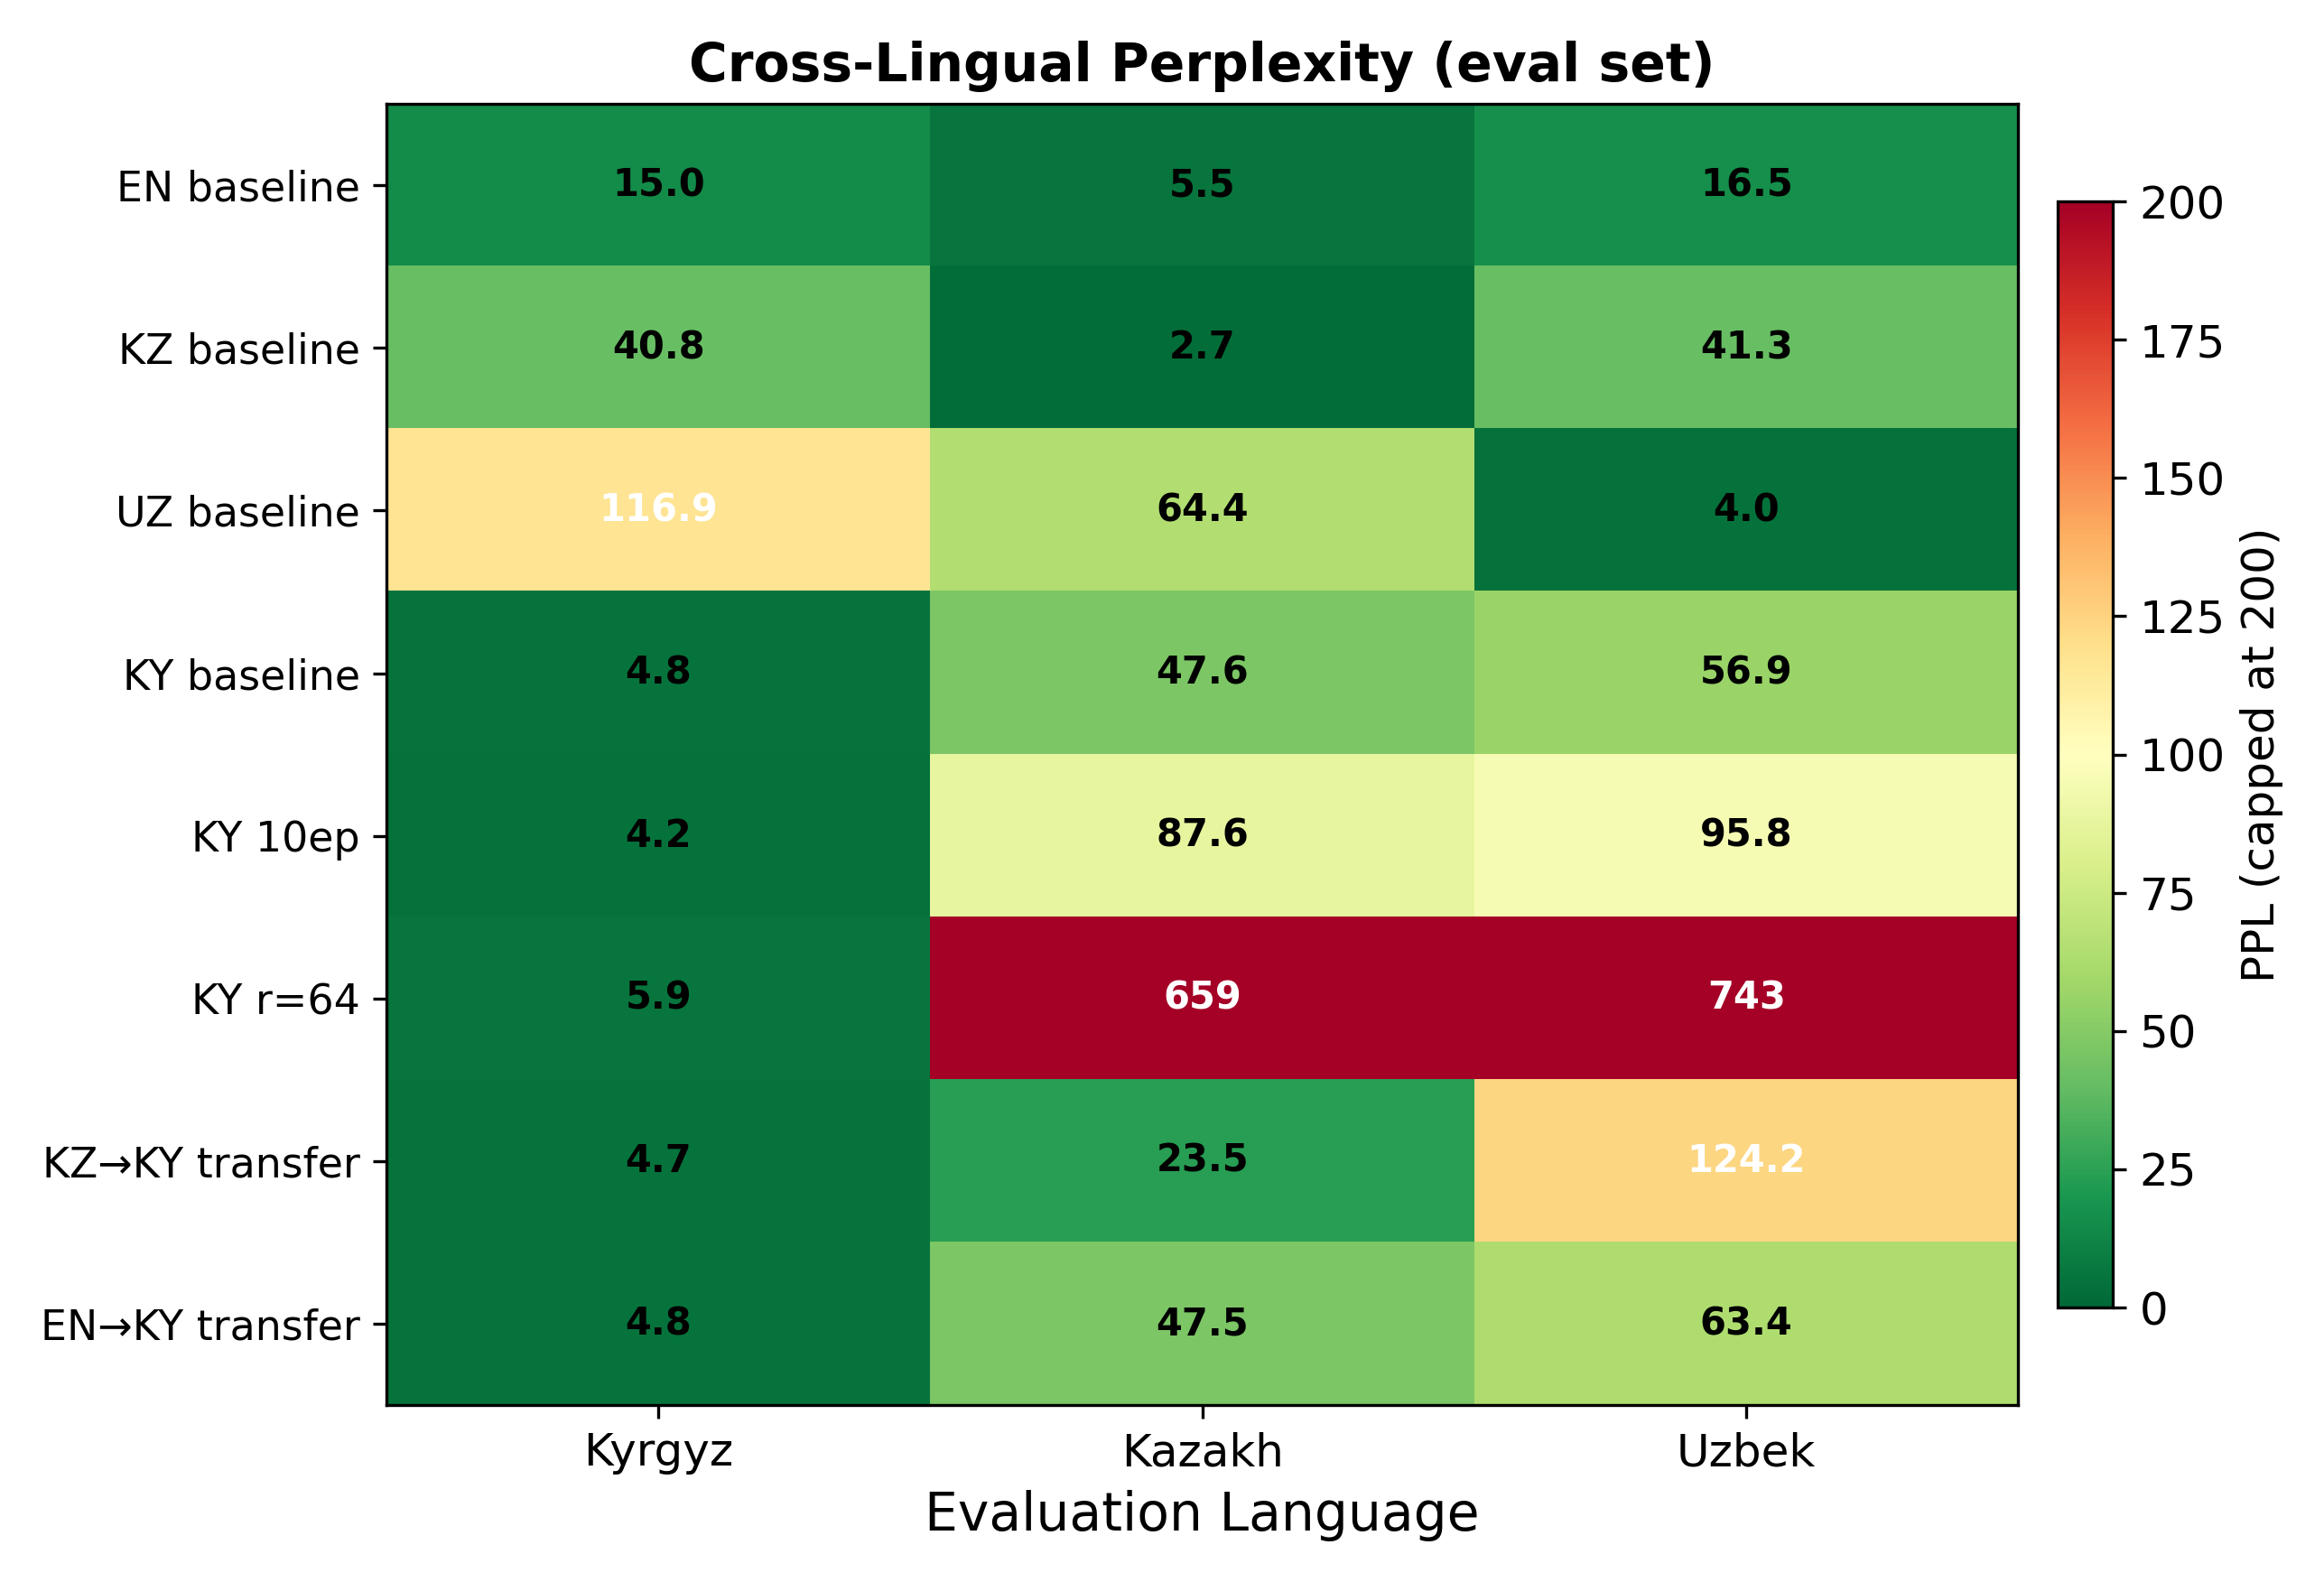
\includegraphics[width=0.75\textwidth]{../figures/fig4_cross_ppl.png}
    \caption{Cross-lingual perplexity heatmap. Darker cells indicate higher perplexity (more forgetting). The $r{=}64$ row is clearly pathological, while the KZ$\rightarrow$KY transfer row shows the most balanced profile.}
    \label{fig:cross_ppl}
\end{figure*}

Critically, the \textbf{EN control experiment} (E8) reveals that Frobenius norm growth alone does not predict forgetting. Despite exhibiting 33$\times$ norm growth---comparable to the KZ baseline (38$\times$)---the EN adapter induces minimal Turkic language degradation (KZ PPL 5.54 vs.\ 47.58 for the KY baseline). This demonstrates that forgetting severity depends not only on the magnitude of weight perturbations but also on their \emph{alignment} with pretrained representations.

\subsection{Spectral Dynamics: Challenging H1}
\label{sec:spectral}

Our central finding is that the spectral energy threshold of 0.7 proposed by \citet{biderman2024lora} is \textbf{never reached} in any of our experiments, including those exhibiting severe functional degradation. \Cref{fig:svd_dynamics} shows the evolution of mean and maximum SE across training steps.

\begin{figure*}[t]
    \centering
    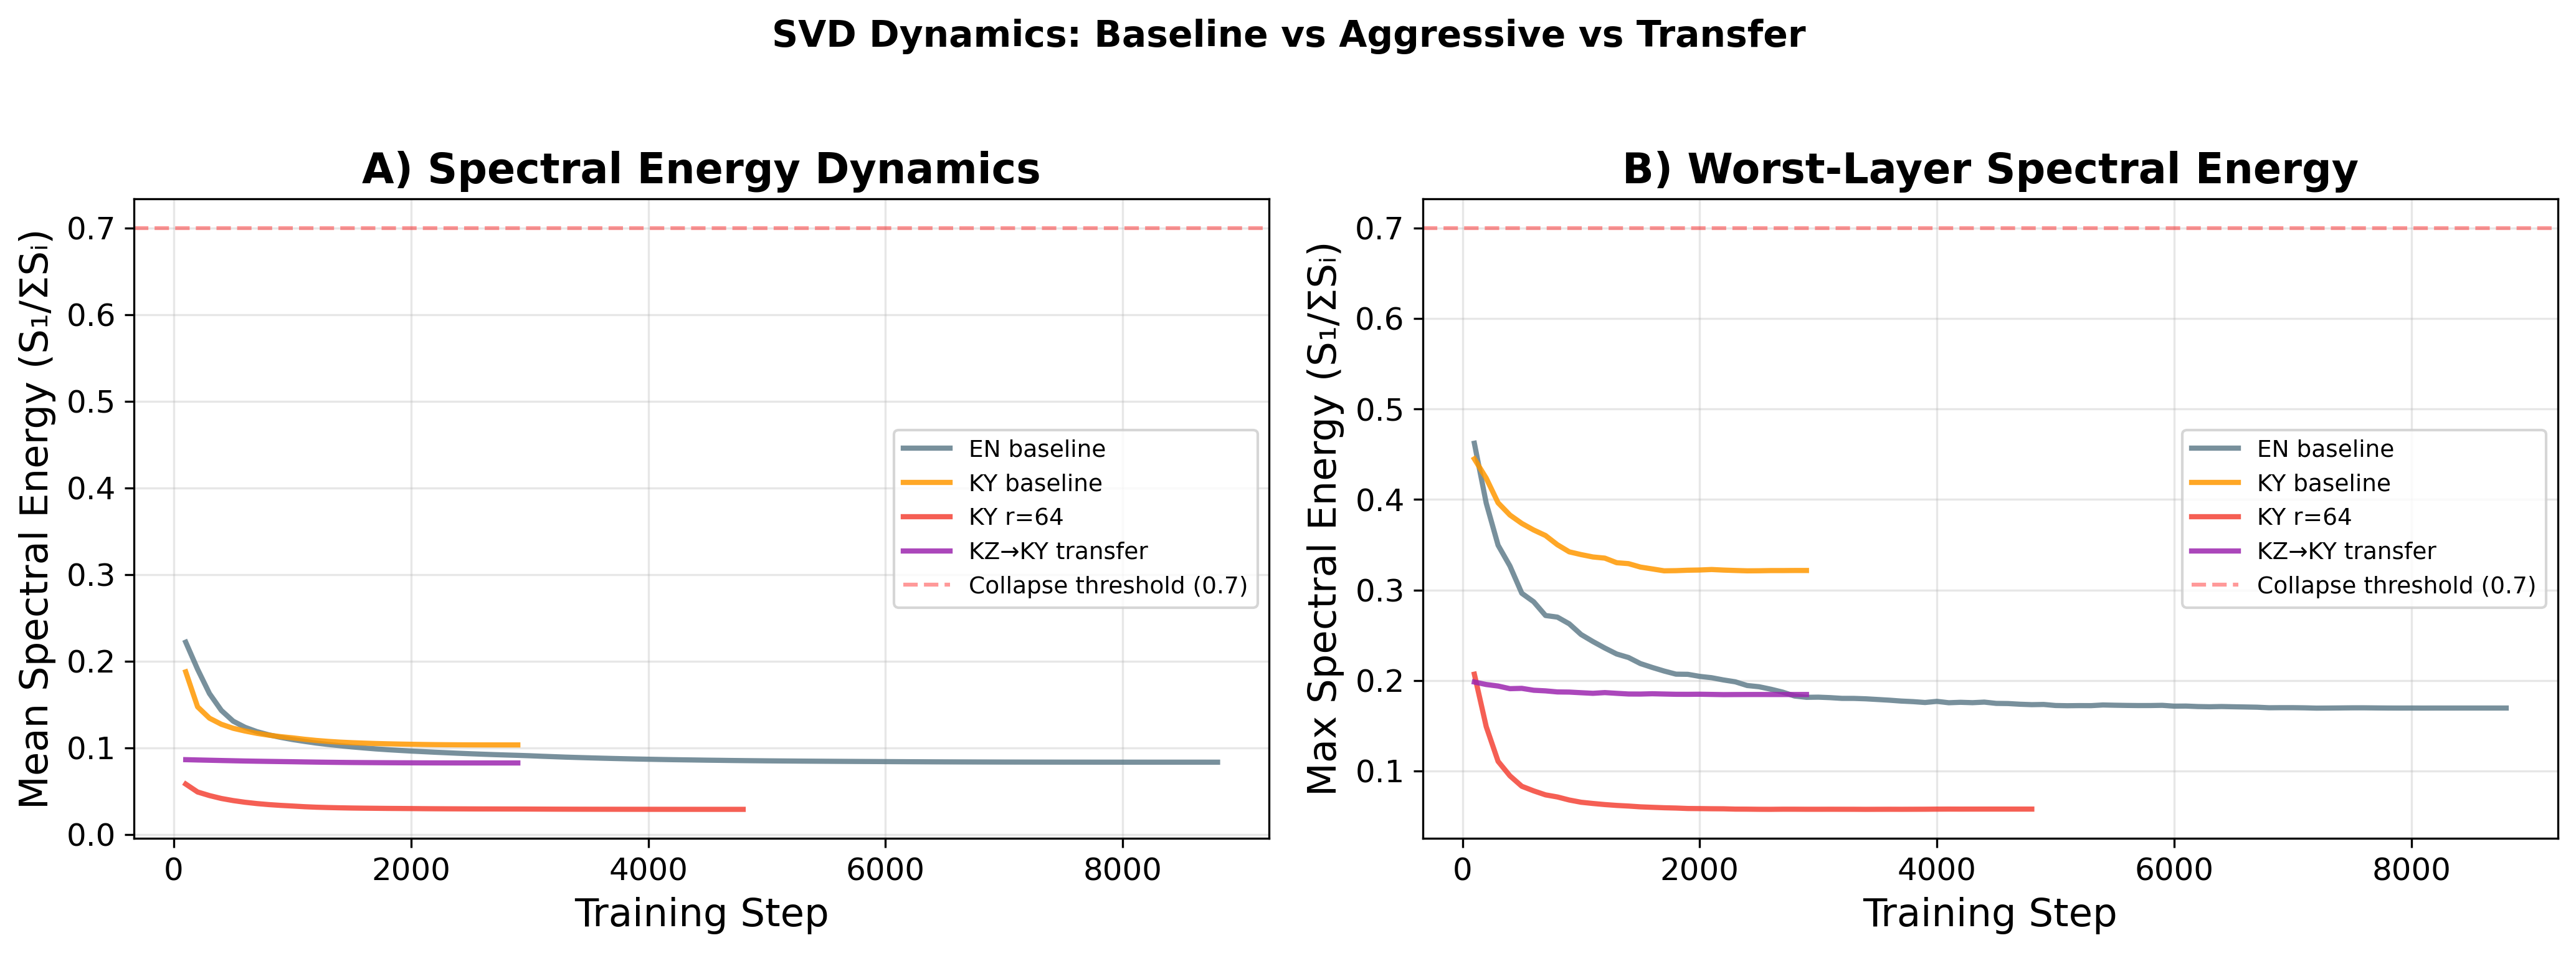
\includegraphics[width=\textwidth]{../figures/fig2_svd_dynamics.png}
    \caption{Spectral energy dynamics during training. Top: mean SE across all layers. Bottom: maximum SE across layers. No experiment approaches the proposed 0.7 threshold. The $r{=}64$ configuration shows \emph{decreasing} SE despite suffering the worst functional degradation.}
    \label{fig:svd_dynamics}
\end{figure*}

The KY baseline ($r{=}16$) shows a mild increase in maximum SE from approximately 0.44 to 0.59, well below the 0.7 threshold. More strikingly, the pathological $r{=}64$ configuration exhibits \emph{decreasing} SE throughout training, from 0.21 to 0.10--0.13. This counterintuitive pattern arises because SE is a \emph{shape} metric: as training progresses, all singular values grow, but growth is distributed across multiple directions, causing the relative contribution of $\sigma_1$ to decrease. The effective rank correspondingly \emph{increases} from approximately 6 to 26 (\Cref{app:effrank}), signaling healthy dynamics under standard interpretations---yet this same configuration suffers complete NER failure.

\Cref{fig:layer_heatmap} confirms that no individual layer approaches the collapse threshold. \textbf{H1 is not supported in our setting:} SE below 0.7 does \emph{not} guarantee healthy training. The fundamental limitation is that SE is a shape metric invariant to rescaling---a weight matrix with singular values $[100, 50, 25]$ and one with $[0.001, 0.0005, 0.00025]$ have identical SE despite vastly different perturbation magnitudes. For higher-rank configurations, SE is additionally \emph{rank-biased}: since $\text{SE} \approx 1/r$ at initialization, higher-rank adapters appear spectrally healthier by definition.

\begin{figure*}[t]
    \centering
    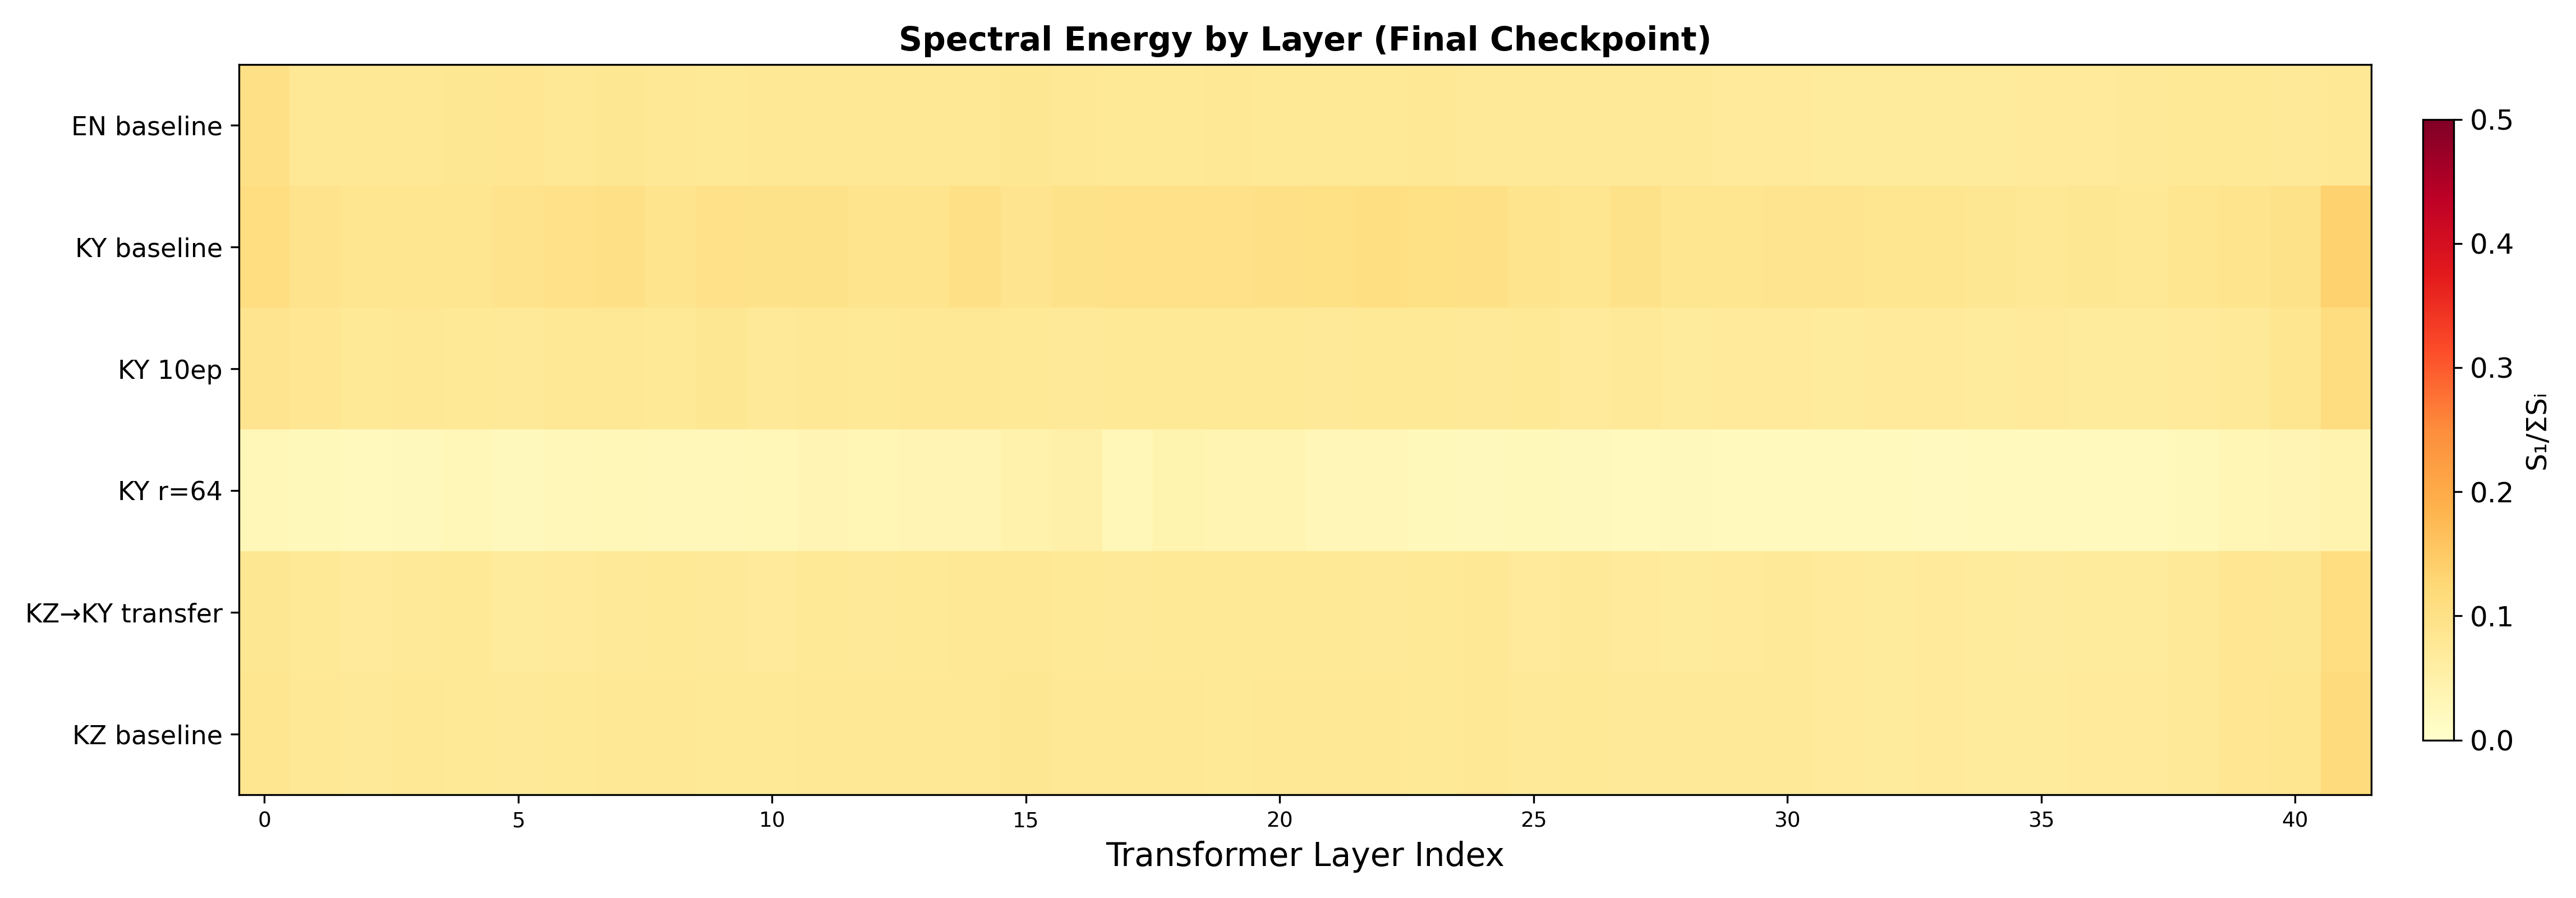
\includegraphics[width=\textwidth]{../figures/fig3_layer_heatmap.png}
    \caption{Layer-wise spectral energy at the final training checkpoint. Each row is an experiment; each column is a transformer layer. No layer in any experiment exceeds the 0.7 threshold.}
    \label{fig:layer_heatmap}
\end{figure*}

\subsection{Frobenius Norm: The Missing Diagnostic}
\label{sec:frobenius}

We find that the \textbf{Frobenius norm growth ratio} of the $\texttt{lora\_B}$ matrices provides a clear separation between healthy and pathological training regimes. \Cref{tab:frobenius} shows that the KZ$\rightarrow$KY transfer exhibits only $+13\%$ growth, while the pathological $r{=}64$ configuration shows 15--38$\times$ growth. However, the EN control complicates the picture: despite $\sim$33$\times$ growth, it causes minimal forgetting, revealing that norm growth is a reliable diagnostic \emph{within} a language category but not \emph{across} categories.

\begin{table}[t]
\centering
\small
\begin{tabular}{lccc}
\toprule
\textbf{Experiment} & $\|\mathbf{B}\|_F^{\text{init}}$ & $\|\mathbf{B}\|_F^{\text{final}}$ & \textbf{Growth} \\
\midrule
KZ$\rightarrow$KY Transfer & 3.043 & 3.436 & 1.13$\times$ \\
KY Baseline $r{=}16$ & 0.227 & 1.899 & 8.36$\times$ \\
EN Control $r{=}16$ & 0.092 & 3.076 & 33.4$\times$ \\
KZ Baseline $r{=}16$ & 0.081 & 3.107 & 38.5$\times$ \\
KY $r{=}64$ & 0.566 & 8.859 & 15.6$\times$ \\
Diverged $r{=}64$ & --- & --- & explodes \\
\bottomrule
\end{tabular}
\caption{Frobenius norm growth ratios for $\texttt{lora\_B}$ matrices. EN control and KZ baseline show comparable growth ($\sim$33--38$\times$), yet EN produces minimal forgetting while KY baseline with only 8$\times$ growth causes severe forgetting---demonstrating that language representation in the pretrained model modulates the impact of weight perturbations.}
\label{tab:frobenius}
\end{table}

\begin{figure*}[t]
    \centering
    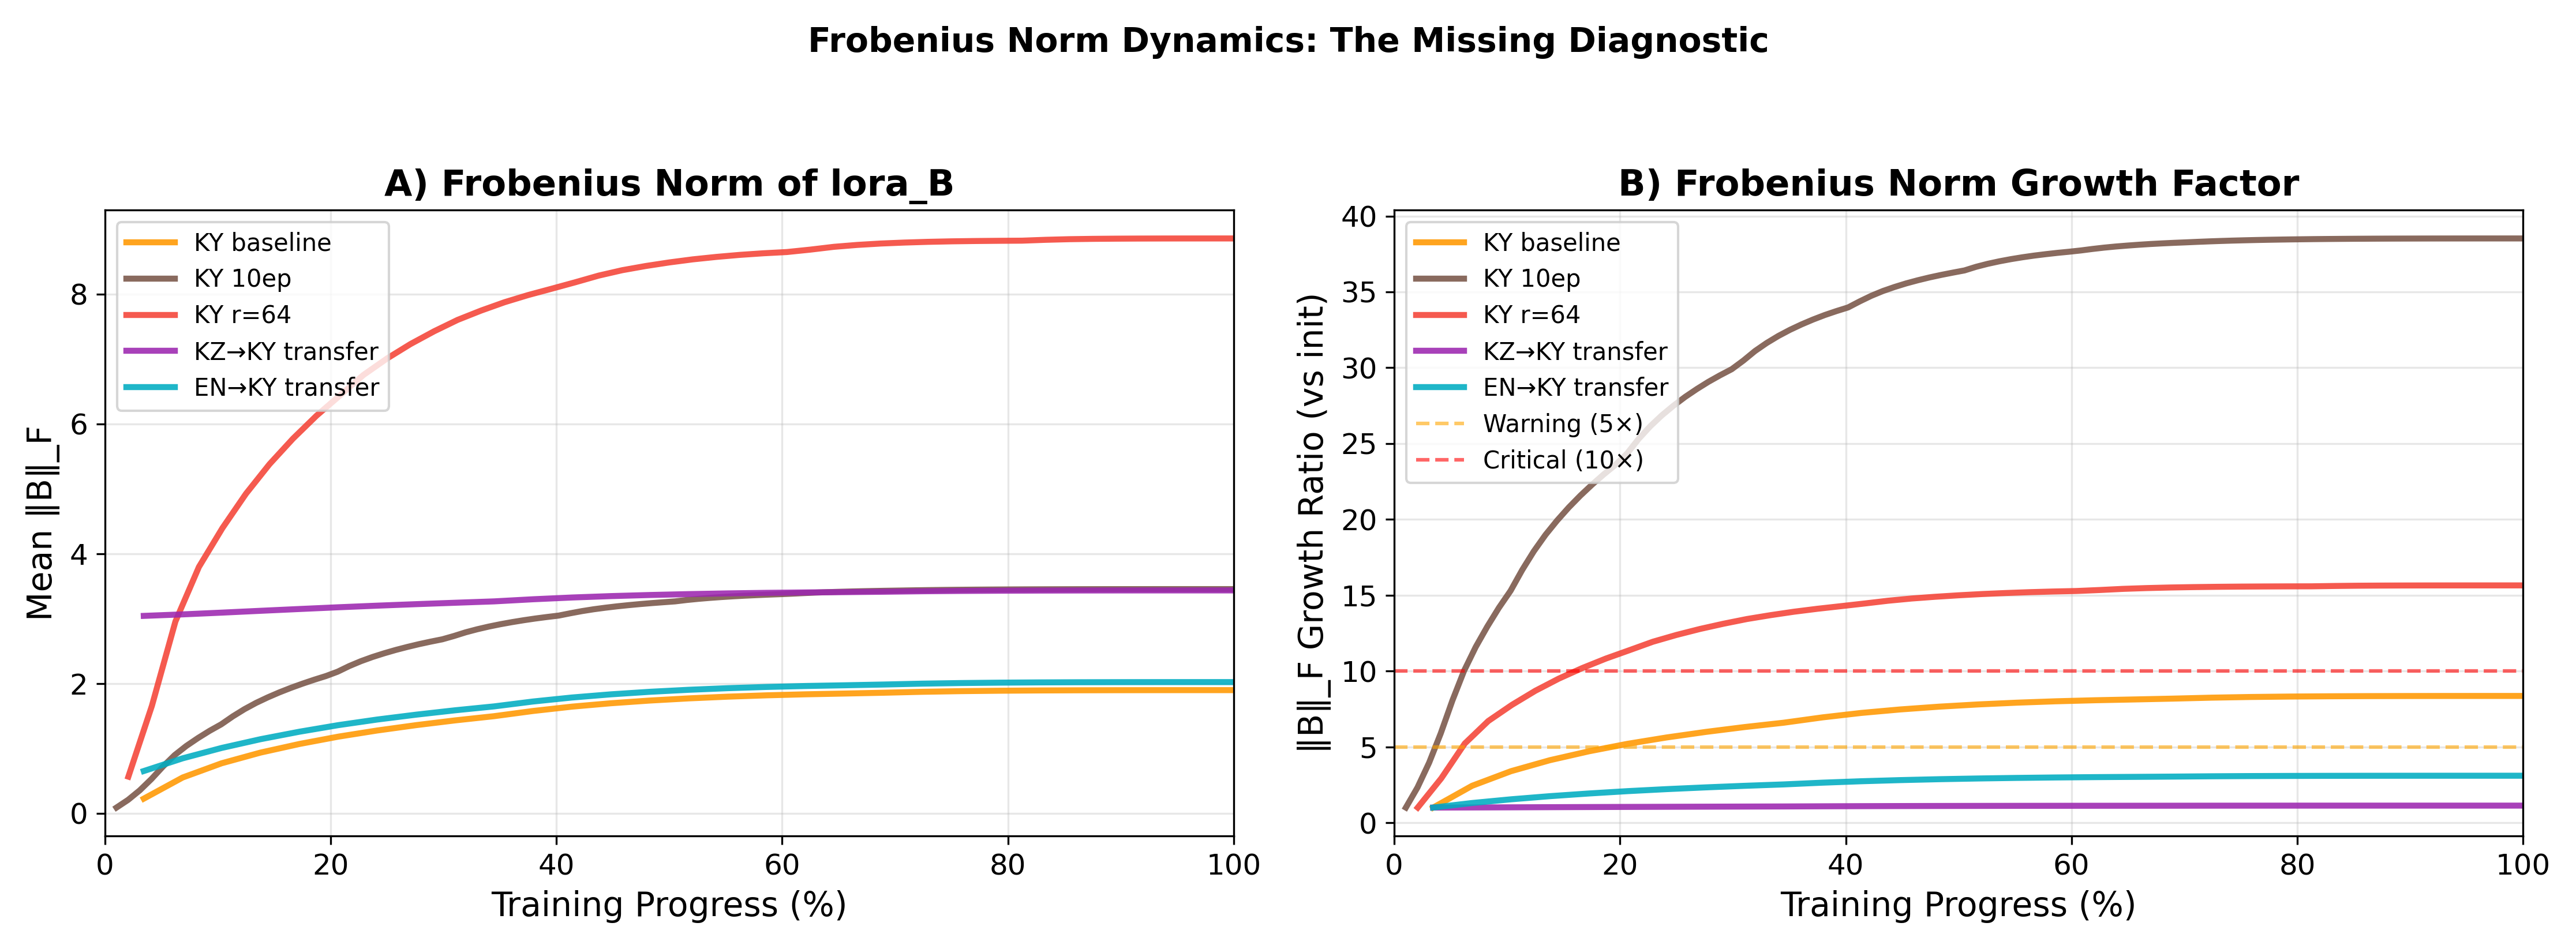
\includegraphics[width=\textwidth]{../figures/fig6_frobenius_dynamics.png}
    \caption{Frobenius norm dynamics of $\texttt{lora\_B}$ matrices during training. The $r{=}64$ configuration shows dramatically larger norm growth compared to $r{=}16$ baselines. The transfer experiment begins at the KZ baseline's final norm and shows minimal additional growth.}
    \label{fig:frobenius}
\end{figure*}

The Frobenius norm captures the \emph{scale} of weight perturbations that SE discards, but the \emph{direction} of those updates---whether they reinforce or disrupt pretrained representations---determines their downstream impact. We propose preliminary growth thresholds ($<2\times$: healthy; 2--10$\times$: normal; $>10\times$: warning) as coarse guidelines, with important caveats discussed in \Cref{app:thresholds}.

\subsection{Cross-Lingual Transfer}
\label{sec:transfer}

The KZ$\rightarrow$KY transfer experiment (E6) initializes LoRA adapters from the final Kazakh checkpoint before continuing training on Kyrgyz data. \Cref{tab:transfer} shows substantial improvements: Kyrgyz NER F1 improves by $+61\%$ (0.253 vs.\ 0.157), target-language PPL is essentially identical (4.73 vs.\ 4.78), and Kazakh knowledge is substantially better retained (KZ PPL 23.49 vs.\ 47.58).

\begin{table}[t]
\centering
\small
\begin{tabular}{lcc}
\toprule
\textbf{Metric} & \textbf{KY Baseline} & \textbf{KZ$\rightarrow$KY} \\
\midrule
PPL (KY) & 4.78 & 4.73 \\
PPL (KZ) & 47.58 & 23.49 \\
PPL (UZ) & 56.85 & 124.19 \\
NER F1 (KY) & 0.157 & 0.253 \\
NER F1 (KZ) & 0.190 & 0.130 \\
NER F1 (UZ) & 0.326 & 0.348 \\
TUMLU (KY) & 34.7\% & 33.7\% \\
TUMLU (KZ) & 30.2\% & 31.7\% \\
$\|B\|_F$ growth & 8.36$\times$ & 1.13$\times$ \\
\bottomrule
\end{tabular}
\caption{Comparison of direct Kyrgyz training (E3) and Kazakh$\rightarrow$Kyrgyz transfer (E6). Transfer improves KY NER F1 by $+61\%$ and retains KZ knowledge (PPL 23.49 vs.\ 47.58). However, UZ PPL increases (124.19 vs.\ 56.85), suggesting the benefit is primarily between closely related Kipchak languages.}
\label{tab:transfer}
\end{table}

However, Uzbek PPL degrades substantially (124.19 vs.\ 56.85), suggesting that sequential transfer between closely related languages (Kazakh and Kyrgyz, both Kipchak-branch, Cyrillic-script) can \emph{harm} more distant relatives (Uzbek, Karluk-branch, historically Latin-script).

\textbf{H2 is partially confirmed:} cross-lingual transfer improves downstream performance and retains source-language knowledge, but the mechanism appears to be \emph{better initialization} rather than \emph{slower degradation}. The transfer adapter begins with an already-trained weight configuration (Frobenius norm growth of only $+13\%$), requiring minimal additional adaptation. Related-language pretraining acts as a \emph{spectral regularizer}: by providing a warm-start with already-structured singular value distributions, it constrains subsequent weight updates to a low-perturbation regime that preserves multilingual knowledge.

% ============================================================================
% 5. ANALYSIS AND DISCUSSION
% ============================================================================
\section{Analysis and Discussion}

\paragraph{Why SE fails.} The failure of the SE threshold stems from LoRA initialization: standard LoRA initializes $B$ with zeros, so after the first gradient update $B$ acquires small singular values with $\text{SE} \approx 1/r$. As training progresses, growth is distributed across multiple directions, causing SE to remain stable or decrease. For $r{=}64$, the SE denominator includes more singular values, mechanically driving SE lower ($1/64 \approx 0.016$ vs.\ $1/16 = 0.0625$), making higher-rank adapters appear healthier by definition---a dangerous trap for practitioners monitoring SE across different rank configurations.

\paragraph{Directionality matters.} The EN control experiment reveals that the critical factor in forgetting is not the \emph{magnitude} of weight updates but their \emph{directionality}. English fine-tuning reinforces already well-represented features with minimal cross-lingual interference, while Turkic fine-tuning forces the model to restructure underrepresented regions of the weight space, disrupting shared multilingual features. This is compounded by the 3.2$\times$ subword fragmentation: Turkic sentences require $\sim$3$\times$ more tokens, reducing the information density per gradient update and forcing larger weight modifications (see \Cref{app:fragmentation}).

\paragraph{The overfit paradox.} Extended training (10 epochs, E4) \emph{improves} target-language PPL (4.18 vs.\ 4.78) despite clear overfitting, but at a steep cost in cross-lingual knowledge (KZ PPL nearly doubles). This suggests a regime of ``useful overfitting'' where the model memorizes target-language patterns more deeply at the expense of multilingual competence. Full analysis is provided in \Cref{app:overfit}.

% ============================================================================
% 6. LIMITATIONS
% ============================================================================
\section{Limitations}

Our study has several important limitations. First, all experiments use a single base model (Gemma-2-9B); results may differ for other architectures. Second, while the EN control uses a matched corpus size, differences in data distribution and tokenizer coverage may partially confound the comparison. Third, NER evaluation relies on few-shot prompting, introducing noise from instruction-following variation. Fourth, we examine only three of $\sim$35 Turkic languages, excluding Turkish. Fifth, experiment E5 ($r{=}64$) simultaneously increases both rank and learning rate relative to baselines, confounding these factors; a controlled $r{=}64$, $\text{lr}{=}2 \times 10^{-4}$ experiment would be needed to isolate rank effects. Sixth, our SVD monitoring focuses on $\texttt{lora\_B}$ matrices; $\texttt{lora\_A}$ dynamics may reveal complementary patterns. Seventh, 4-bit quantization may influence spectral properties in ways not captured by our analysis. Eighth, our Frobenius norm thresholds are derived from a single experimental setting and should be treated as preliminary guidelines. Finally, our Uzbek corpus is restricted to Cyrillic-script sources; since Uzbekistan officially uses Latin script and most contemporary formal text is Latin-based, our Uzbek results may not generalize to Latin-script data.

% ============================================================================
% 7. CONCLUSION
% ============================================================================
\section{Conclusion}

We have presented a systematic study of the spectral dynamics of LoRA adapters during fine-tuning on three low-resource Turkic languages, yielding three principal findings. First, the spectral energy threshold hypothesis is \textbf{not supported}: no experiment exceeds SE of 0.59, yet $r{=}64$ configurations suffer complete functional collapse. Second, \textbf{Frobenius norm growth ratio} is a useful but language-dependent diagnostic---it reliably separates healthy from pathological regimes within underrepresented languages, but well-represented languages absorb comparable growth without degradation. Third, \textbf{sequential cross-lingual transfer} between related Turkic languages is highly effective: KZ$\rightarrow$KY transfer improves NER F1 by $+61\%$ while retaining Kazakh knowledge.

Based on these findings, we recommend that practitioners: (1) monitor Frobenius norm growth rather than spectral energy; (2) avoid aggressive rank--LR combinations for small corpora; (3) use related-language transfer when available; (4) apply cross-lingual perplexity monitoring as a forgetting diagnostic; and (5) consider early stopping by cross-lingual PPL rather than training loss.

Future work should validate these findings across diverse architectures (particularly in full-precision BF16), extend the analysis to additional Turkic languages, and investigate directional norm regularization as a training objective.

% ============================================================================
% ETHICS STATEMENT
% ============================================================================
\section*{Ethics Statement}

This work involves fine-tuning language models on text corpora from three Turkic languages and English. While we aim to improve NLP capabilities for underserved language communities, we acknowledge that language models can amplify biases present in training data. Our training corpora, drawn from Wikipedia, literary texts, and web sources, may contain cultural biases or factual inaccuracies.

\textbf{Data availability:} The Kazakh and Uzbek corpora are compiled from publicly available sources. The Kyrgyz corpus is curated from licensed sources and cannot be redistributed. We release all trained LoRA adapters, SVD monitoring logs, evaluation results, and full training code, enabling complete reproduction of the evaluation and analysis stages.

% ============================================================================
% ACKNOWLEDGMENTS
% ============================================================================
\section*{Acknowledgments}

We thank the creators of the Kazakh, Kyrgyz, and Uzbek corpora used in this study, as well as the developers of the TUMLU benchmark. All experiments were conducted on personal hardware without external funding.

\paragraph{LLMs Usage Statement.} During the preparation of this manuscript, we made limited use of large language models (LLMs), specifically Anthropic's Claude, to assist with language refinement and organization of some sections. All technical content, equations, derivations, and experimental design were developed entirely by the authors. The LLM was not used for ideation of methods, data analysis, or generation of results.

% ============================================================================
% REPRODUCIBILITY
% ============================================================================
\section*{Reproducibility Statement}

All experimental code (training with SVD monitoring, evaluation, and plotting scripts), fine-tuned LoRA adapters for all eight experiments, SVD monitoring logs, and evaluation reports are publicly available at \url{https://anonymous.4open.science/r/Spectral-Collapse-Turkic-EMNLP-7D8F}. The Kazakh, Uzbek, and English training corpora are derived from publicly available sources and can be reconstructed using the provided data preparation scripts. The Kyrgyz corpus cannot be redistributed due to licensing restrictions; however, the released KY adapters and SVD logs enable full reproduction of all evaluation and analysis stages.

% ============================================================================
% REFERENCES
% ============================================================================
\bibliography{references}

\appendix

% ============================================================================
% APPENDIX
% ============================================================================

\section{SVD Metric Definitions}
\label{app:metrics}

\textbf{Spectral Energy (SE)} quantifies the dominance of the largest singular value:
\begin{equation}
    \text{SE} = \frac{\sigma_1}{\sum_{i=1}^{r} \sigma_i}
\end{equation}

\textbf{Effective Rank} \cite{roy2007effective} measures the number of significantly contributing singular values:
\begin{equation}
    \text{EffRank} = \exp\left(-\sum_{i=1}^{r} p_i \log p_i\right), \quad p_i = \frac{\sigma_i}{\sum_j \sigma_j}
\end{equation}

\textbf{Stable Rank} provides a continuous relaxation of matrix rank:
\begin{equation}
    \text{StableRank} = \frac{\|W\|_F^2}{\sigma_1^2} = \frac{\sum_i \sigma_i^2}{\sigma_1^2}
\end{equation}

\textbf{SVD Entropy} measures the uniformity of the singular value distribution:
\begin{equation}
    H_{\text{SVD}} = -\sum_{i=1}^{r} p_i \log_2 p_i
\end{equation}

\textbf{Frobenius Norm} captures the overall magnitude of the weight matrix:
\begin{equation}
    \|W\|_F = \sqrt{\sum_{i=1}^{r} \sigma_i^2}
\end{equation}

\section{Detailed Training Configurations}
\label{app:configs}

All experiments were conducted on a single NVIDIA GeForce RTX 5080 (16~GB) using PyTorch 2.10, Transformers 5.2, and PEFT 0.18. \Cref{tab:training_details} provides the full training statistics.

\begin{table}[H]
\centering
\scriptsize
\begin{tabular}{llcccc}
\toprule
\textbf{ID} & \textbf{Experiment} & \textbf{Train} & \textbf{Eval} & \textbf{Eval} & \textbf{Time} \\
 & & \textbf{Loss} & \textbf{Loss} & \textbf{PPL} & \textbf{(min)} \\
\midrule
E1 & KZ Baseline & 0.275 & 1.259 & 3.52 & 477 \\
E2 & UZ Baseline & 1.193 & 1.822 & 6.18 & 341 \\
E3 & KY Baseline & 0.815 & 1.920 & 6.82 & 183 \\
E4 & KY Overfit & 1.050 & 1.963 & 7.12 & 1193 \\
E5 & KY $r{=}64$ & 0.274 & 2.164 & 8.71 & 157 \\
E6 & KZ$\rightarrow$KY & 1.809 & 1.932 & 6.90 & 355 \\
E8 & EN Control & 1.821 & 2.017 & 7.51 & 1351 \\
\bottomrule
\end{tabular}
\caption{Full training statistics. Eval loss and PPL are computed on the validation split during training. The higher train loss for E6 reflects the adapter starting from KZ-optimized weights.}
\label{tab:training_details}
\end{table}

\section{Cross-Lingual Perplexity Matrix}
\label{app:cross_ppl}

\begin{table}[H]
\centering
\small
\begin{tabular}{lccc}
\toprule
\textbf{Trained on} & \textbf{KY PPL} & \textbf{KZ PPL} & \textbf{UZ PPL} \\
\midrule
KZ Baseline & 40.75 & \textbf{2.73} & 41.27 \\
UZ Baseline & 116.89 & 64.44 & \textbf{4.03} \\
KY Baseline & \textbf{4.78} & 47.58 & 56.85 \\
KY Overfit & \textbf{4.18} & 87.65 & 95.76 \\
KY $r{=}64$ & 5.90 & 659.25 & 742.73 \\
KZ$\rightarrow$KY & 4.73 & 23.49 & 124.19 \\
\midrule
EN Control & 14.96 & 5.54 & 16.55 \\
\bottomrule
\end{tabular}
\caption{Cross-lingual perplexity matrix. Each row is an adapter; each column is the evaluation language. Bold indicates target-language PPL. The $r{=}64$ configuration shows catastrophic cross-lingual degradation ($>600\times$ PPL increase), while the EN control shows minimal Turkic forgetting despite comparable Frobenius norm growth (33$\times$).}
\label{tab:cross_ppl}
\end{table}

\section{Frobenius Norm Growth Thresholds}
\label{app:thresholds}

Our experiments suggest the following practical thresholds for $\|B\|_F$ growth monitoring:
\begin{itemize}
    \item $< 2\times$: \textbf{Healthy} training; minimal forgetting (e.g., transfer setup: 1.13$\times$).
    \item $2$--$10\times$: \textbf{Normal} training; moderate forgetting expected (e.g., KY baseline: 8.36$\times$).
    \item $> 10\times$: \textbf{Warning}; significant forgetting likely (e.g., $r{=}64$: 15--38$\times$).
    \item Unbounded growth: \textbf{Training failure}; divergence imminent (e.g., E7).
\end{itemize}

These thresholds refer to \emph{relative growth} (ratio of final to initial Frobenius norm). \textbf{Important caveats:} The KZ baseline (E1, 38.5$\times$) and EN control (E8, 33.4$\times$) both exceed the $>10\times$ warning threshold without functional collapse, while the KY baseline (E3, 8.36$\times$) falls within the ``normal'' range yet shows significant cross-lingual forgetting. We recommend these thresholds as coarse guidelines rather than precise decision boundaries.

\section{Effective Rank Dynamics}
\label{app:effrank}

\Cref{fig:effrank} shows the effective rank dynamics across experiments. The $r{=}64$ configuration shows increasing effective rank (from $\sim$6 to $\sim$26), indicating growing parameter utilization. The diverged experiment (E7) is the only configuration where effective rank \emph{decreases} (from 43.3 to 37.1), consistent with true spectral collapse.

\textbf{E7 divergence analysis.} The diverged experiment ($r{=}64$, $\text{lr}{=}10^{-3}$) provides the most extreme datapoint. Training terminated at step 800 due to loss divergence. Even at this point, maximum SE was only 0.18---still far below the 0.7 threshold---while mean Frobenius norm had already reached 6.75 (19$\times$ growth in just 800 steps). The Frobenius norm shows clear exponential growth from step 100 onward, providing a much earlier warning signal than SE.

\begin{figure}[H]
    \centering
    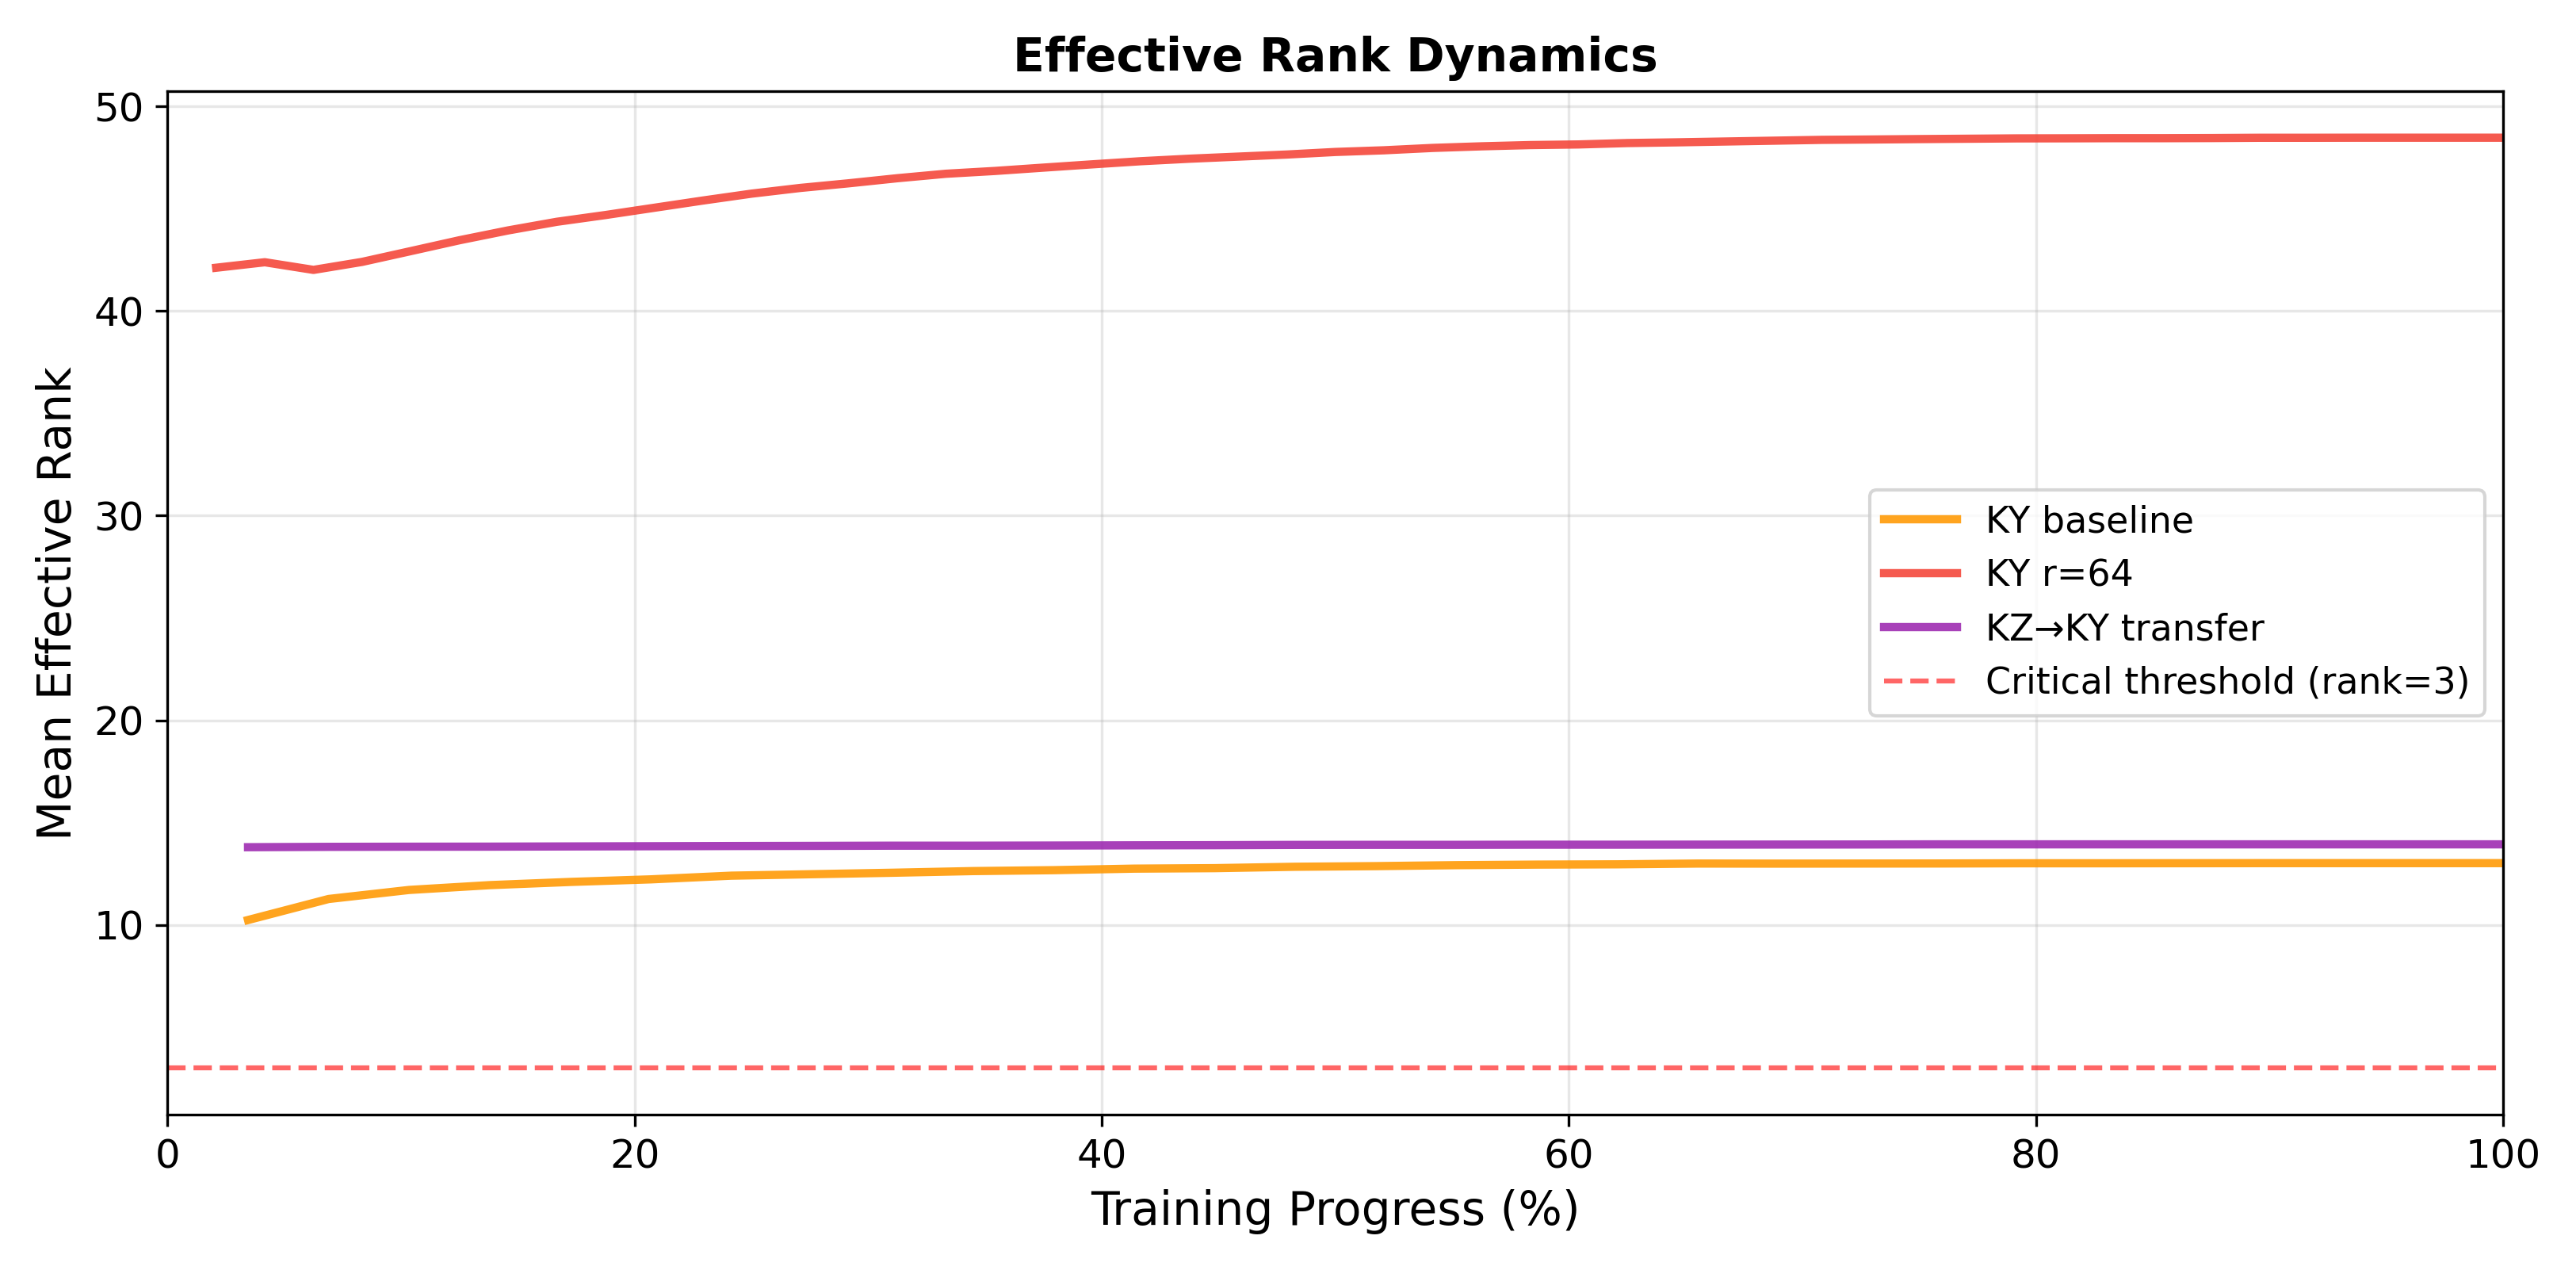
\includegraphics[width=\columnwidth]{../figures/fig5_effective_rank.png}
    \caption{Effective rank dynamics during training. The $r{=}64$ configuration shows increasing effective rank despite functional degradation, further evidence that standard spectral metrics can be misleading.}
    \label{fig:effrank}
\end{figure}

\section{The Overfit Paradox}
\label{app:overfit}

The 10-epoch Kyrgyz experiment (E4) reveals a paradoxical pattern (\Cref{fig:overfit}): extended training \emph{improves} target-language perplexity (4.18 vs.\ 4.78 for the 3-epoch baseline) despite clear indicators of overfitting (final train loss 0.165 vs.\ 0.815 for the baseline). However, this improvement comes at a steep cost in cross-lingual knowledge: Kazakh PPL nearly doubles (87.65 vs.\ 47.58), Uzbek PPL increases by 68\% (95.76 vs.\ 56.85), and TUMLU accuracy on Kazakh drops from 30.2\% to 27.8\%. The spectral profile remains healthy throughout (SE $< 0.5$), further confirming that SE is not a reliable indicator of training pathology.

\begin{figure}[H]
    \centering
    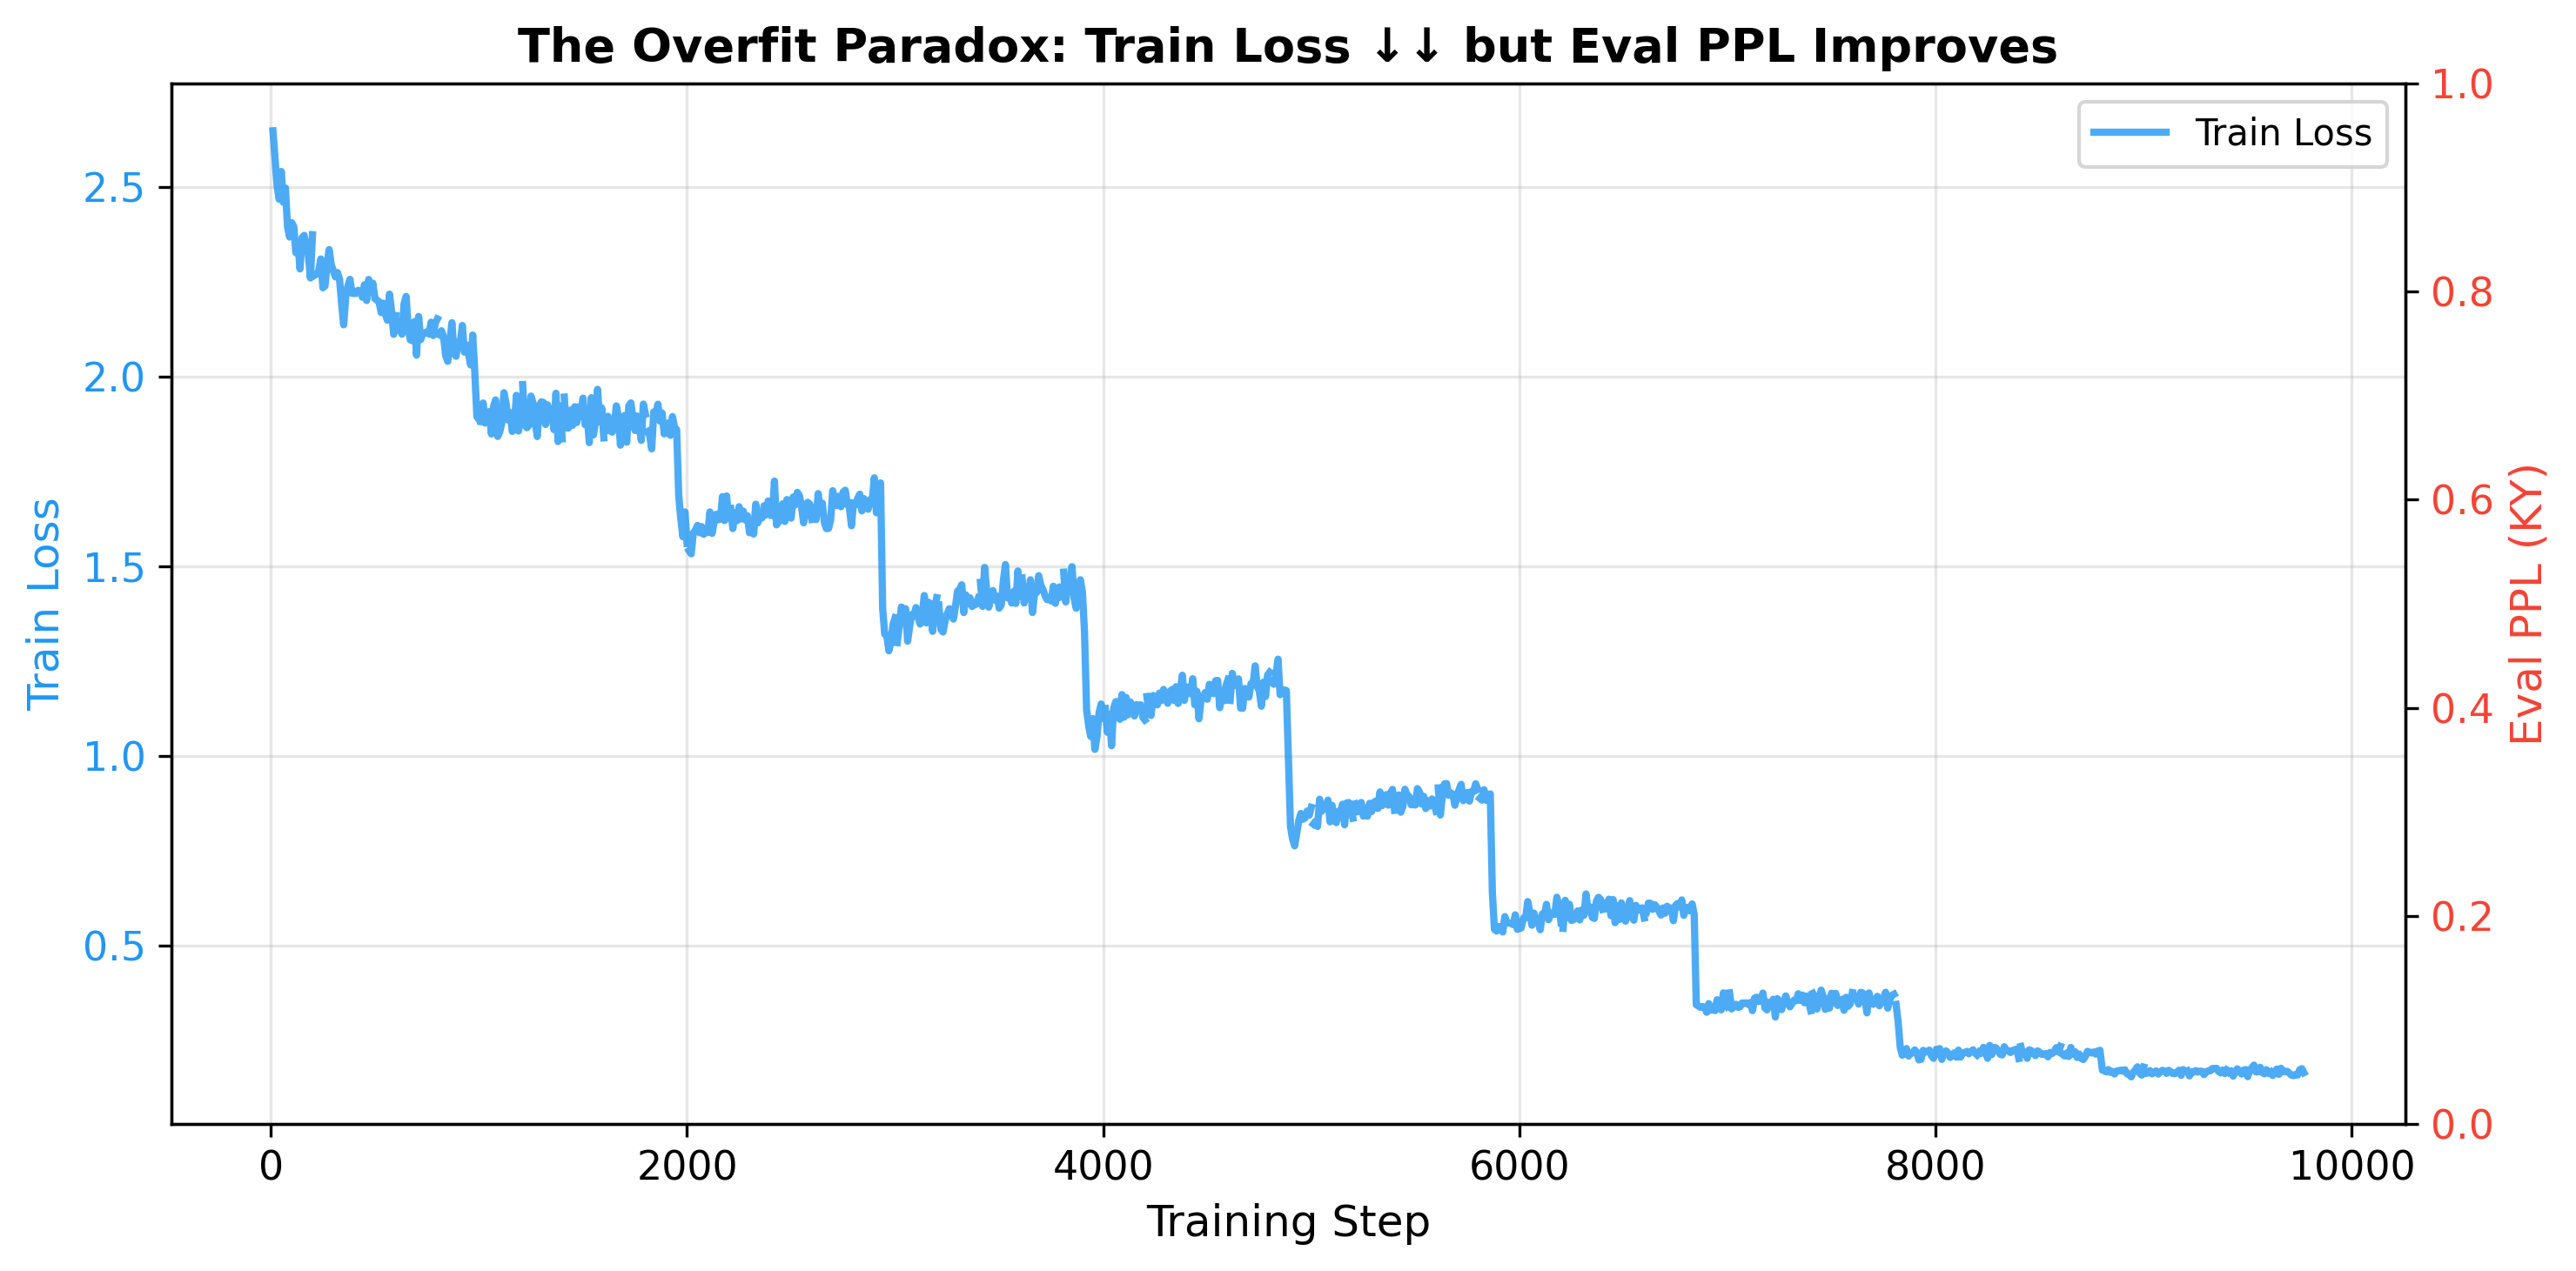
\includegraphics[width=\columnwidth]{../figures/fig7_overfit_paradox.png}
    \caption{The overfit paradox: 10 epochs of Kyrgyz training (E4) yields better target-language PPL (4.18 vs.\ 4.78) despite increasing cross-lingual degradation. Train loss continues to decrease while cross-lingual PPL rises monotonically.}
    \label{fig:overfit}
\end{figure}

\section{Role of Subword Fragmentation}
\label{app:fragmentation}

\begin{table}[H]
\centering
\small
\begin{tabular}{lcc}
\toprule
\textbf{Language} & \textbf{Tokens/Word} & \textbf{Ratio to EN} \\
\midrule
English & 1.15 & 1.00$\times$ \\
Uzbek & 3.68 & 3.20$\times$ \\
Kyrgyz & 3.69 & 3.21$\times$ \\
Kazakh & 3.74 & 3.25$\times$ \\
\bottomrule
\end{tabular}
\caption{Subword fragmentation ratios for the Gemma-2-9B tokenizer.}
\label{tab:tokenization}
\end{table}

The 3.2$\times$ subword fragmentation ratio has several compounding effects on LoRA adaptation:

\textbf{Sequence length inflation:} A Kyrgyz sentence of 50 words requires approximately $50 \times 3.69 = 185$ tokens, versus $50 \times 1.15 = 58$ tokens for English. With a maximum sequence length of 256 tokens, each training example contains substantially less textual content, reducing the information density of each gradient update.

\textbf{Morphological fragmentation:} Agglutinative suffixes carrying grammatical meaning are split across multiple subwords, forcing the model to reconstruct morphological relationships across token boundaries.

\textbf{Link to forgetting severity:} The EN control provides direct evidence that subword fragmentation interacts with forgetting dynamics. Despite comparable Frobenius norm growth (EN: 33$\times$ vs.\ KZ: 38$\times$), the EN adapter causes minimal cross-lingual degradation while Turkic adapters cause severe forgetting, suggesting that the critical factor is the \emph{directionality} of weight updates rather than their magnitude.

\section{Singular Value Distributions}
\label{app:svd_dist}

\begin{figure}[H]
    \centering
    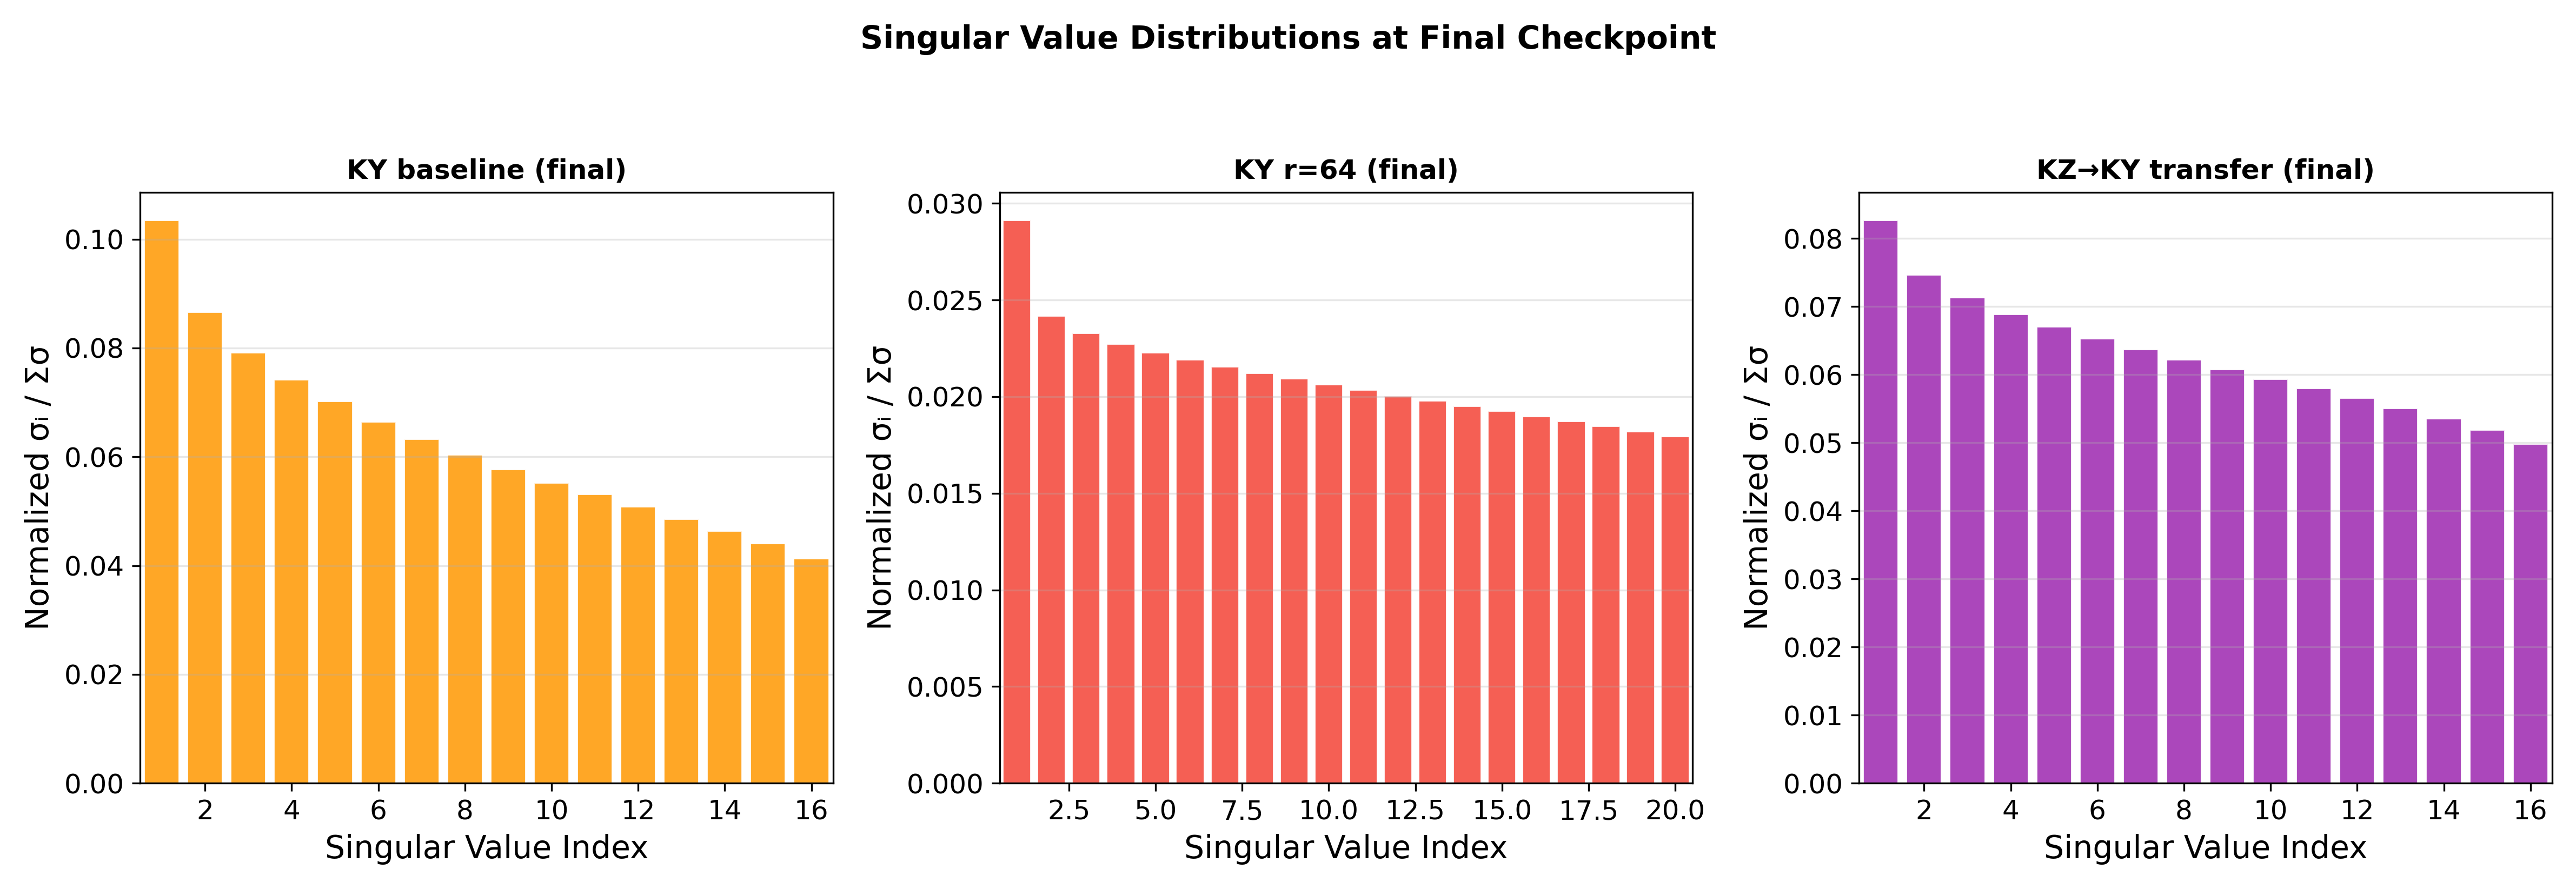
\includegraphics[width=\columnwidth]{../figures/fig8_singular_values.png}
    \caption{Singular value distributions at the final checkpoint. The $r{=}64$ configuration (right) shows a well-distributed spectrum (low SE) with dramatically larger absolute magnitudes compared to the $r{=}16$ baseline (left), explaining why SE fails to detect pathological training.}
    \label{fig:singular_values}
\end{figure}

\section{Frobenius Norm vs.\ Cross-Lingual PPL}
\label{app:scatter}

\begin{figure}[H]
    \centering
    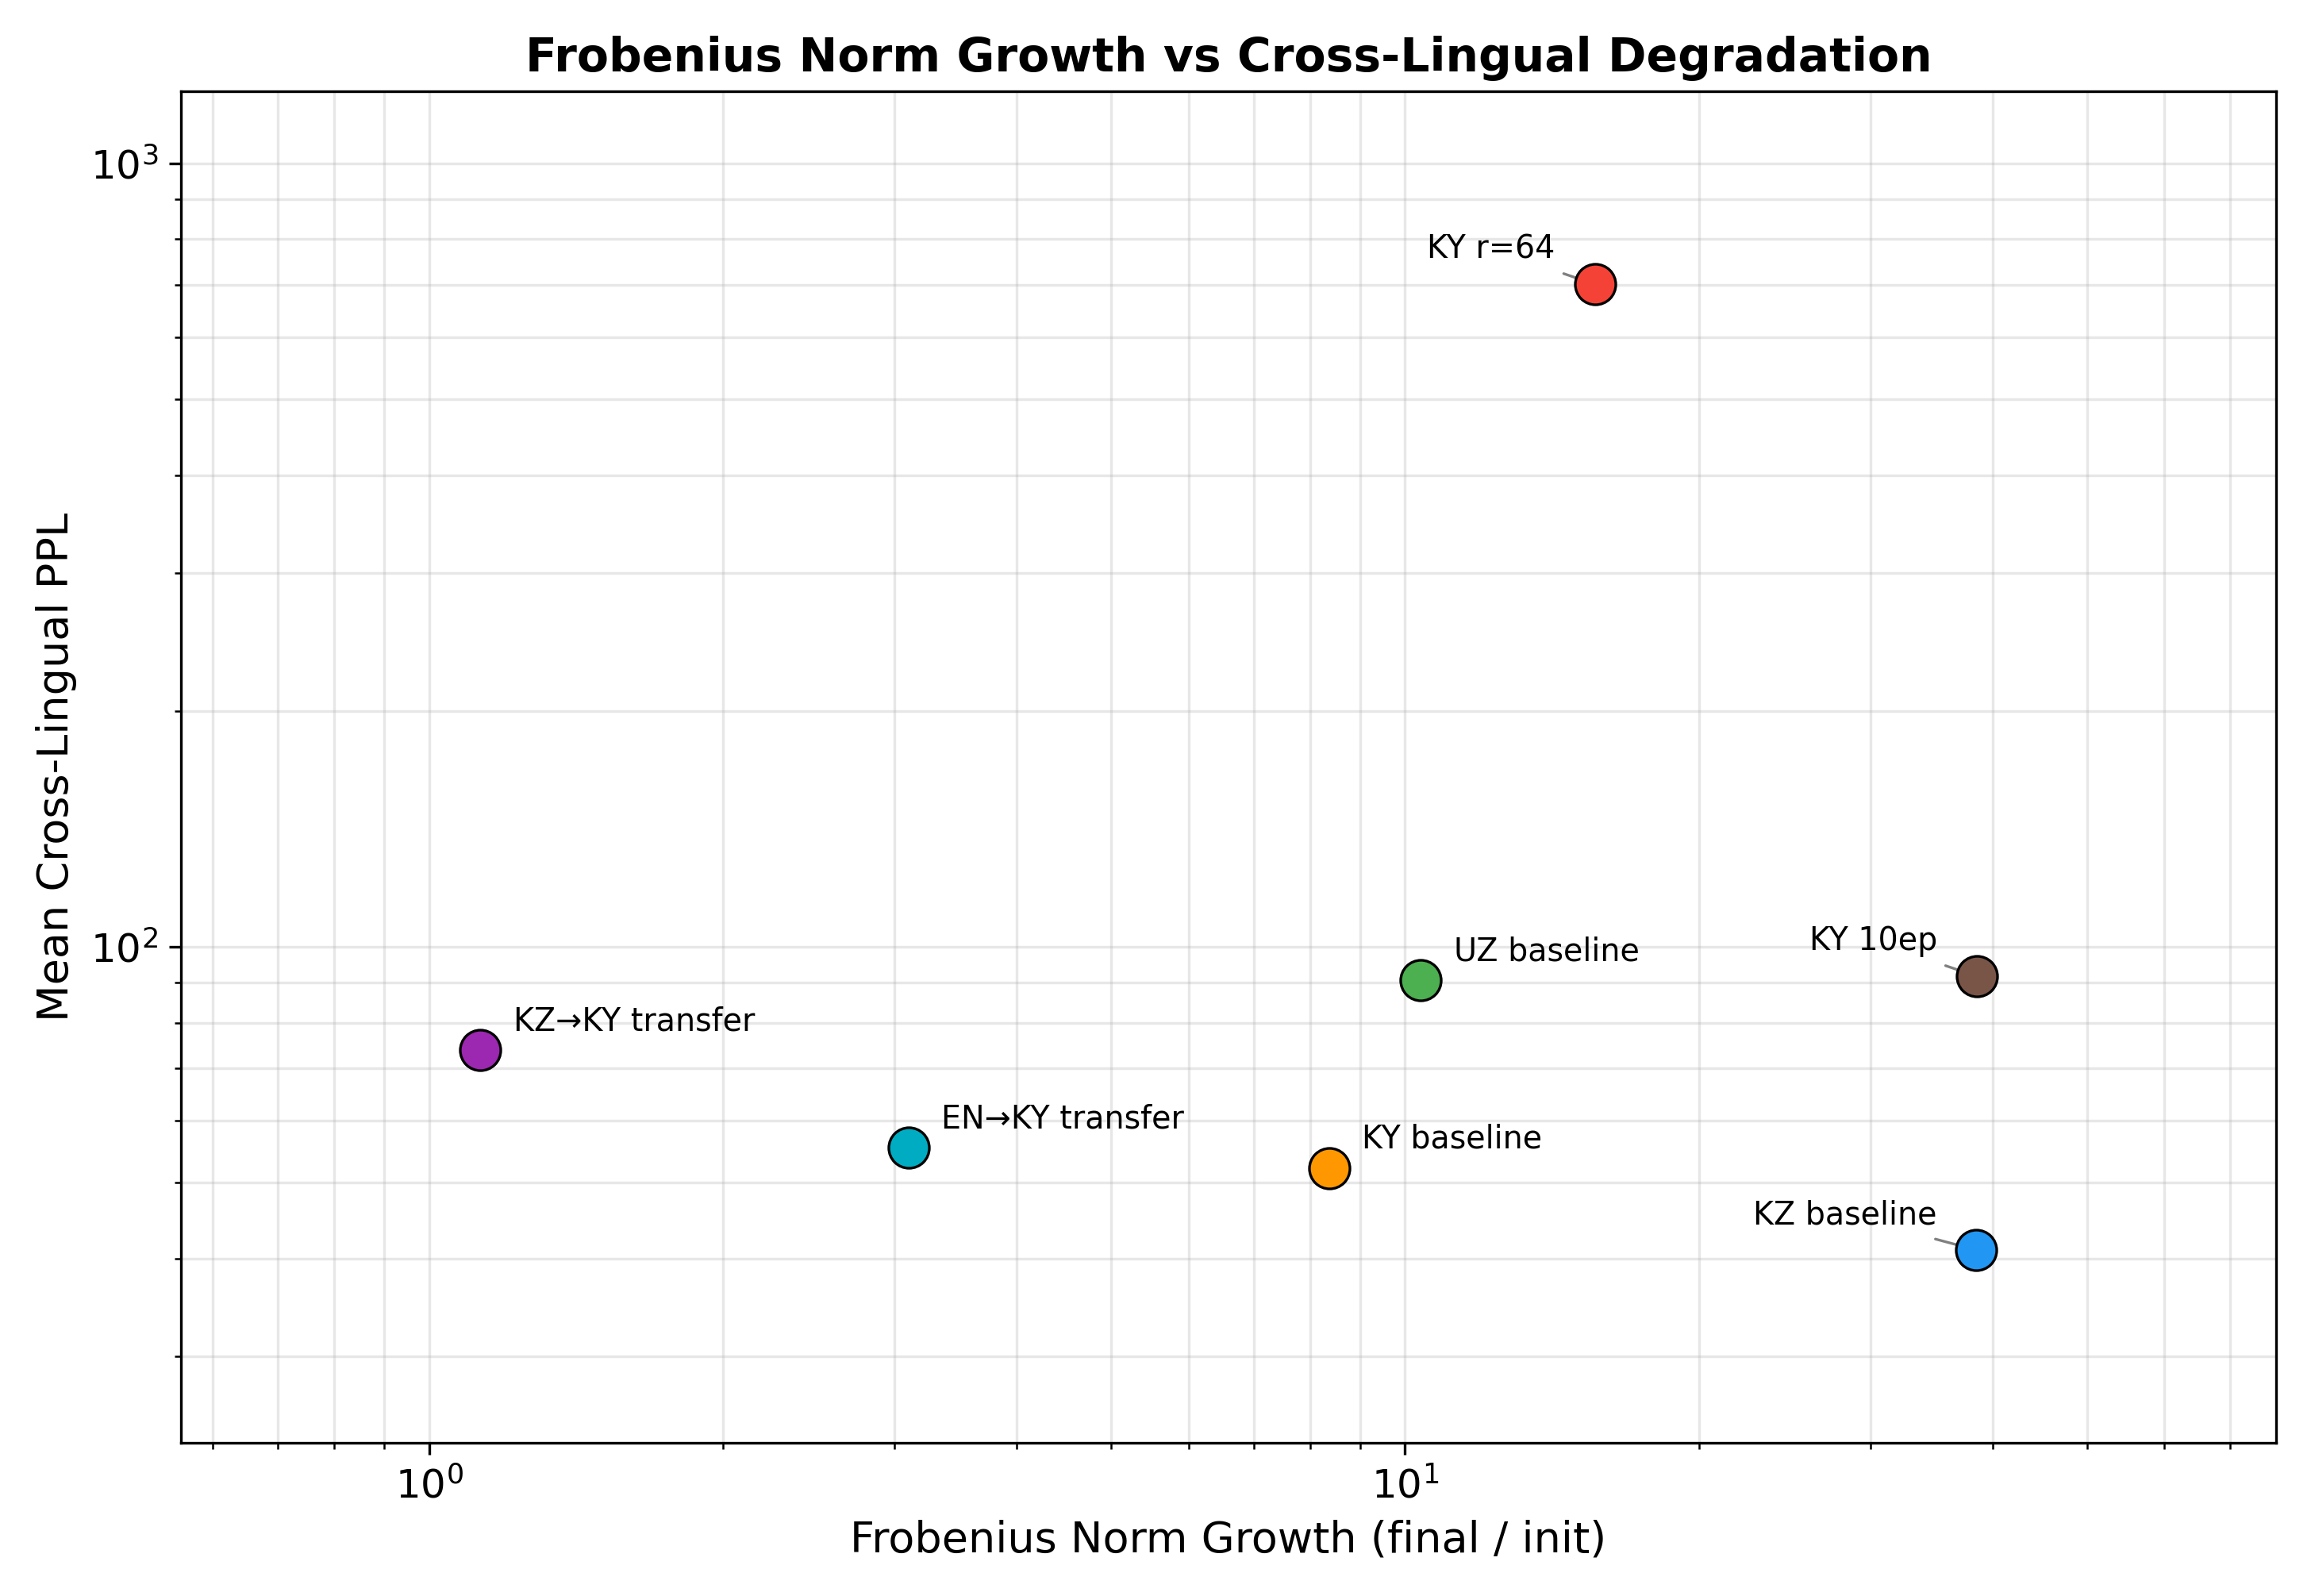
\includegraphics[width=\columnwidth]{../figures/fig9_frobnorm_vs_ppl.png}
    \caption{Frobenius norm growth ratio versus cross-lingual perplexity degradation. Within Turkic experiments, the pattern is monotonically consistent ($\rho_s = 0.26$, $n{=}6$). The EN control is a clear outlier (33$\times$ growth with minimal forgetting), confirming that norm growth is necessary but not sufficient for catastrophic forgetting.}
    \label{fig:frobnorm_scatter}
\end{figure}

\section{Detailed Evaluation Results}
\label{app:ner}

\Cref{tab:ner_pertype} breaks down NER performance by entity type. \Cref{tab:tumlu_full} presents TUMLU accuracy across all languages.

\begin{table}[H]
\centering
\small
\begin{tabular}{lccc}
\toprule
\textbf{Experiment} & \textbf{PER F1} & \textbf{ORG F1} & \textbf{LOC F1} \\
\midrule
KZ Baseline (on KY) & 0.236 & 0.162 & 0.229 \\
UZ Baseline (on KY) & 0.095 & 0.150 & 0.209 \\
KY Baseline & 0.101 & 0.160 & 0.266 \\
KY Overfit & 0.224 & 0.255 & 0.119 \\
KY $r{=}64$ & 0.000 & 0.000 & 0.000 \\
KZ$\rightarrow$KY & 0.344 & 0.202 & 0.214 \\
\bottomrule
\end{tabular}
\caption{Per-type NER F1 scores on Kyrgyz WikiANN. The KZ$\rightarrow$KY transfer achieves the highest PER F1 (0.344). The $r{=}64$ configuration produces zero scores due to 100\% parse failures.}
\label{tab:ner_pertype}
\end{table}

\begin{table}[H]
\centering
\small
\begin{tabular}{lccc}
\toprule
\textbf{Experiment} & \textbf{KY} & \textbf{KZ} & \textbf{UZ} \\
\midrule
KZ Baseline & 35.7\% & 38.4\% & 32.8\% \\
UZ Baseline & 31.9\% & 33.1\% & 35.4\% \\
KY Baseline & 34.7\% & 30.2\% & 29.6\% \\
KY Overfit & 33.9\% & 27.8\% & 31.5\% \\
KY $r{=}64$ & 23.2\% & 22.2\% & 22.9\% \\
KZ$\rightarrow$KY & 33.7\% & 31.7\% & 30.8\% \\
\bottomrule
\end{tabular}
\caption{TUMLU accuracy across all experiments and languages. The $r{=}64$ configuration drops to near-random levels ($\sim$23\%) across all languages.}
\label{tab:tumlu_full}
\end{table}

\noindent\textbf{Functional collapse examples.}
To illustrate functional collapse at $r{=}64$, we present raw model outputs. The model ignores instructions and exhibits degenerate repetition.

{\small
\textbf{NER prompt:} \texttt{Extract named entities from the text. Format each as: ENTITY ||| TYPE}

\textbf{Input:} {\cyrfont\textit{Бишкекте Кыргыз Республикасынын Президенти Садыр Жапаров менен Казакстандын Президенти Касым-Жомарт Токаев жолукту.}}

\textbf{$r{=}64$ output:} {\cyrfont\textit{Кыргыз Республикасынын Президентинин кызматына кандидат болгон. Кыргыз Республикасынын Президентинин кызматына кандидат болгон. Кыргыз Республикасынын Президентинин кызматына кандидат болгон\ldots}} (repeats indefinitely)

\textbf{Text continuation prompt:} {\cyrfont\textit{Кыргызстан --- это}}

\textbf{$r{=}64$ output:} {\cyrfont\textit{не только, не только, не только, не только, не только\ldots}} (single bigram repeated 25+ times until max tokens)

Both examples demonstrate complete loss of instruction-following capability---degenerate repetitions are a hallmark of functional collapse distinct from spectral collapse.
}

\end{document}
